% HWP 양식 결과보고서 LaTeX 원고 (제안모형 C-BAT 기준). 빌드: tectonic main.tex
\documentclass[11pt,a4paper]{article}
\usepackage[top=22mm,bottom=22mm,left=22mm,right=22mm]{geometry}
\usepackage{kotex}
\setmainhangulfont{Noto Serif CJK KR}
\setsanshangulfont{Noto Sans CJK KR}
\XeTeXlinebreaklocale ""
\usepackage{amsmath,amssymb,bm}
\usepackage{array,booktabs,longtable,graphicx,caption,etoolbox}
\usepackage{tikz}
\usepackage[hyphens]{url}
\usepackage[hidelinks]{hyperref}

\graphicspath{{../report/figs/}}

% 줄간격 1.5 내외(LaTeX 1.3 = 한글 문서의 1.5배 줄간격에 해당), 단락 첫 줄 들여쓰기 1em
\linespread{1.3}
\setlength{\parindent}{1em}
\setlength{\parskip}{0.2ex}
\renewcommand{\tablename}{표}
\renewcommand{\figurename}{그림}
\captionsetup{font=small,labelsep=period,skip=4pt}
\captionsetup[table]{position=top}
\renewcommand{\arraystretch}{1.1}
\newcolumntype{L}[1]{>{\raggedright\arraybackslash}p{#1}}
\newcommand{\hwptablefont}{\small\linespread{1.12}\selectfont}

% □ 제N장. 제목〔배점점〕 — 장마다 새 쪽. 배점이 없으면 세 번째 인자를 비운다.
\newcommand{\hwpchapter}[3]{%
  \clearpage
  \noindent{\bfseries\large □ 제#1장. #2\ifblank{#3}{}{〔#3점〕}}\par\vspace{0.8ex}}
% 번호 없는 절 제목(번호는 직접 쓴다): \hwpsection{1.1 분석 대상 및 주요 변수}
\newcommand{\hwpsection}[1]{%
  \par\vspace{1.2ex plus 0.5ex}\noindent{\bfseries #1}\par\nopagebreak\vspace{0.3ex}}
% 작은 글씨 "* " 주석 단락
\newcommand{\hwpnote}[1]{%
  \par\begingroup\footnotesize\setlength{\parindent}{0pt}\hangindent=1em\hangafter=1
  * #1\par\endgroup}
% 각 항목 앞에 "-"를 붙인 들여쓰기 목록
\newenvironment{hwplist}{%
  \begin{list}{-}{\setlength{\leftmargin}{2em}\setlength{\labelwidth}{1em}%
    \setlength{\labelsep}{0.6em}\setlength{\itemsep}{0.2ex}%
    \setlength{\topsep}{0.3ex}\setlength{\parsep}{0pt}}}{\end{list}}

\begin{document}
% placeholder: 표지 (Task 6에서 작성)

\hwpchapter{1}{데이터 이해 및 진단}{15}

\hwpsection{1.1 분석 대상 및 주요 변수}

KAMP 자원 최적화 AI 데이터셋(\texttt{okm\_augumented\_2021.csv})으로 생산조건에 따른 전력과 일 피크를 분석하였다. 한 공장의 시간별 생산량, 전력, 기상 기록이며 2021년 1월 1일부터 9월 14일까지 257일, 하루 24행씩 모두 6,168행과 18개 열로 이루어져 있다. 한 행에 그 시간의 15분 단위 전력 네 값(15분·30분·45분·60분 열)이 들어 있어 이를 펼치면 하루 96개, 모두 24,672개의 15분 슬롯이 된다. 예측 대상은 이 슬롯의 전력이며, 하루 96개 값의 최댓값을 일 피크(일 최대전력)로 정의하였다.

원자료를 직접 열어 확인한 내용은 다음과 같다. 결측은 풍속 3행, 강수량 1행, 공장인원 17행에만 있고 나머지 열에는 없다. 전력은 0--222 범위이며 0값이 74개 있다(1.3절). 생산량은 0--9,830이고 3,511행이 양수, 2,657행이 0이며, 257일 가운데 64일은 하루 종일 생산량이 0이다. \texttt{day}, \texttt{d}, \texttt{m} 열은 각각 요일(1=월요일, 7=일요일), 일, 월이며 6,168행 모두 날짜 열에서 얻는 값과 같다. 열별 형태와 이 보고서에서의 사용 방식은 표~\ref{tab:ch1-vars}에 정리하였다.

{\hwptablefont
\setlength{\tabcolsep}{4pt}
\begin{longtable}{L{2.2cm}L{3.3cm}L{4.0cm}L{5.7cm}}
\caption{원자료의 열과 사용 방식.}\label{tab:ch1-vars}\\
\toprule
원자료 열 & 형태·범위 & 공정상 의미 & 사용 \\
\midrule
\endfirsthead
\caption[]{원자료의 열과 사용 방식(계속).}\\
\toprule
원자료 열 & 형태·범위 & 공정상 의미 & 사용 \\
\midrule
\endhead
\midrule
\multicolumn{4}{r}{\footnotesize 다음 쪽에 계속}\\
\endfoot
\bottomrule
\endlastfoot
날짜 & 정수(YYYYMMDD). 2021-01-01--09-14, 257일 & 관측일. 하루 24행(시간별) & 예측일 식별. 시간순 분할과 요일·월·공휴일 계산의 기준 \\
시간 & 정수 0--23(48행은 이 범위 밖의 값) & 하루 안의 시각(시) & 슬롯 시각 부여. 7월 13일과 15일의 48행은 값이 어긋나 행 순서로 대체 \\
15분·30분·45분·60분 & 정수 0--222(kW로 해석). 0값 74개 & 공장 전체의 15분 평균전력. 한 행에 그 시간의 네 슬롯 & 평가 목표(하루 96슬롯, 일 피크). C-BAT 입력: 과거 전력(학습 목표, 기준일 곡선). 비교모형 입력: 과거 전력(M2·LightGBM(튜닝)은 시차·요약 변수, B0·B0\_kind는 기준일 곡선) \\
평균 & 정수 0--208 & 네 전력값 평균의 반올림(6,168행 모두 일치) & 제외: 전력에서 계산된 값 \\
생산량 & 정수 0--9,830. 양수 3,511행, 0 2,657행 & 그 시간의 생산 실적. 공정이 돌았는지와 생산 규모 & 실적을 생산계획으로 간주. C-BAT 입력: 시간별 24개 값에서 생산 여부·정규화 로그 생산량·가동유형 산출. 비교모형 입력: M2·LightGBM(튜닝)은 시간별 값·일 합계·생산시간, B0\_kind는 가동유형으로 기준일 선택 \\
기온·풍속·습도·강수량 & 기온 $-12.0$--33.4, 풍속 0.0--7.6, 습도 8--98(정수), 강수량 0.0--122.4(누적). 풍속 3행, 강수량 1행 결측 & 공장 밖의 기상 & C-BAT 제외: 공장 위치를 알 수 없어 기상 예보를 연결할 수 없다. 비교모형 입력: M2·LightGBM(튜닝)은 전일 기온·습도·풍속 평균과 전일 강수 합계만 입력. B0·B0\_kind는 미사용 \\
전기요금(계절) & 실수 세 값: 109.8(1--2월), 167.2(3--5월, 9월), 191.6(6--8월) & 계절별 요금 단가. 한 달 안에서는 일정 & 제외: 예측 입력이 아니다. 비용 분석은 시간대를 구분하는 한국전력 산업용(을) 2021년 요금표로 계산 \\
\texttt{day}·\texttt{d}·\texttt{m} & 정수. day 1--7, d 1--31, m 1--9 & 요일, 일, 월. 하루 24행이 같은 값 & 제외: 날짜 열과 중복. 요일·월은 날짜에서 다시 계산하여 사용 \\
공장인원 & 실수. 17행 결측(전력 네 값이 모두 0인 17개 시간) & 생산량을 한 시간 안 전력 네 값의 합으로 나눈 값. 실제 작업자 수가 아님 & 제외: 목표 전력이 계산에 들어 있어 정보 누수 \\
인건비 & 1.0(2,295행) 또는 1.5(3,873행) & 시각별 인건비 할증 배수. 09--17시 2,313행 중 2,295행이 1.0, 그 밖의 시각은 모두 1.5 & 제외: 예측 입력이 아니며 분석에도 쓰지 않았다 \\
\end{longtable}}
\hwpnote{C-BAT는 이 보고서가 제안하는 모형으로, 시간별 생산계획을 바탕으로 한 조건부 베이지안 전달모형이며 2.1절에서 설명한다. 전력은 kW로 해석하였다. 자료 설명에 단위가 없는 생산량과 기상 열은 값 그대로 사용하였다. 비교모형은 B0(7일 전 전력 곡선), B0\_kind(같은 가동유형의 기준일 곡선), M2(LightGBM 기본), LightGBM(튜닝), 기존 BAT이며 구성은 2장에서 설명한다. 기존 BAT는 C-BAT와 같은 변수를 쓴다.}

원자료에 없는 파생 변수는 표~\ref{tab:ch1-derived}에 정리하였다. 가동유형은 하루에 생산량이 양수인 시간 수로 정하므로 생산계획에서 바로 계산되고, 예측 시점에 알 수 있다.

\begin{table}[htbp]
\hwptablefont
\setlength{\tabcolsep}{4pt}
\caption{원자료에서 만든 파생 변수.}\label{tab:ch1-derived}
\begin{tabular}{L{2.5cm}L{6.4cm}L{6.3cm}}
\toprule
파생 변수 & 정의 & 사용 \\
\midrule
생산 여부 & 시간별 생산량이 양수이면 1, 아니면 0 & C-BAT 입력(생산 여부 채널). M2·LightGBM(튜닝) 입력(슬롯별 생산 여부) \\
정규화 로그 생산량 & $\log(1+q)/\log(1+q_{\max})$. $q$는 시간별 생산량, $q_{\max}$는 학습 기간의 시간별 최대 생산량 & C-BAT 입력(로그 생산량 채널). M2·LightGBM(튜닝)은 정규화하지 않은 생산량 원값 사용 \\
하루 생산시간·일 총생산량 & 생산량이 양수인 시간 수, 시간별 생산량의 합 & M2·LightGBM(튜닝)의 일 피크 모형 입력 \\
가동 여부 & 그날 생산량의 합이 0보다 크면 가동(시각 오류일 2일은 가동으로 표시) & C-BAT 기준일 선택. M2·LightGBM(튜닝) 입력. B0는 7일 전 곡선이 없을 때 대체 기준일 선택에만 사용 \\
가동유형 & 0(0시간)·1(1--12시간)·2(13--19시간)·3(20시간 이상) & C-BAT 입력(유형별 기본 곡선, 가동 상태별 잡음). B0\_kind 기준일 선택. M2·LightGBM(튜닝)은 가동유형 대신 가동 여부와 생산시간 사용 \\
날짜유형 & 평일(월--금), 토요일, 일요일 & C-BAT 기준일 선택. M2·LightGBM(튜닝) 입력. B0\_kind 기준일 선택 \\
요일·월 & 날짜에서 계산(계절은 월에서 계산) & M2·LightGBM(튜닝) 입력. C-BAT 미사용 \\
공휴일 & 2021년 8일(1월 1일, 2월 11--13일, 3월 1일, 5월 5일, 5월 19일, 8월 16일)을 별도 목록으로 관리 & M2·LightGBM(튜닝) 입력. 비용 분석(요금 시간대 판정). C-BAT 미사용 \\
\bottomrule
\end{tabular}
\end{table}
\hwpnote{기존 BAT는 이 표의 C-BAT 입력과 같은 파생 변수(생산 여부, 정규화 로그 생산량, 가동유형, 가동 여부, 날짜유형)를 쓴다.}

정리하면 C-BAT는 예측일의 시간별 생산계획, 예측일 이전의 전력, 가동 여부와 날짜유형만 입력하며 기상, 공휴일, 요일, 월은 쓰지 않았다. M2와 LightGBM(튜닝)은 여기에 달력 정보(요일·월·공휴일)와 전일 기상·전일 생산 요약값을 더하였다.

\hwpsection{1.2 제조공정 상태의 해석}

본 자료는 공장 전체의 생산량과 전력을 집계한 자료이다. 생산시간과 물량 집중에 따른 부하 변화를 분석하는 데에는 적합하나, 개별 설비의 가동 여부, 제품 종류, 교대조 정보가 없어 특정 설비나 공정이 피크를 일으킨 원인은 직접 확정하지 않았다. 하루 종일 생산량이 0인 날에도 전력은 관측되어(비가동일의 일 피크 중앙값 27 kW), 생산 실적이 없는 상태와 설비 전체의 정지를 구분하였다.

생산량이 양수인 시간 수에 따라 하루를 가동유형 0(비가동, 0시간)·1(1--12시간)·2(13--19시간)·3(20시간 이상)으로 구분하였다. 복사일, 시각 오류일, 결측이 있는 날을 제외한 1--8월 완전관측일 117일에서 가동유형별 일 피크의 중앙값은 각각 27, 112, 186, 193 kW였다(표~\ref{tab:ch1-kind}). 생산시간이 긴 유형에서 일 피크가 높았으나 증가 폭은 일정하지 않았고(가동유형 2와 3의 차이는 7 kW), 유형별 범위가 서로 겹쳐 가동유형만으로 일 피크가 정해지지는 않았다. 이에 따라 가동유형으로 운영 상태를 구분하고 시간별 생산량과 과거 전력 곡선을 함께 쓰도록 모형을 구성하였다(2장).

\begin{table}[htbp]
\centering
\hwptablefont
\caption{가동유형별 일 피크(1--8월 완전관측일 117일, kW).}\label{tab:ch1-kind}
\begin{tabular}{L{4.2cm}rrr}
\toprule
가동유형 & 일수 & 중앙값 & 범위 \\
\midrule
0 (비가동, 0시간) & 24 & 27 & 25--116 \\
1 (1--12시간) & 18 & 112 & 104--197 \\
2 (13--19시간) & 22 & 186 & 172--222 \\
3 (20시간 이상) & 53 & 193 & 119--222 \\
\bottomrule
\end{tabular}
\end{table}
\hwpnote{비가동일의 최댓값 116 kW는 1월 2일 하루이며 나머지 23일은 25--31 kW였다. 생산시간은 생산 실적이 기록된 시간 수이며 설비 운전시간이나 교대조 수를 뜻하지 않는다. 유형별 차이는 관측된 연관성으로 해석하였다.}

개발 구간(2021년 7월 7일부터 8월 31일까지를 14일씩 나눈 검증 구간 f1--f4, 1.4절)에서 일 피크를 평가하는 51일 가운데 고피크일은 13일이다. 고피크일은 일 피크가 해당 학습 기간 가동일 일 피크의 90\% 분위수(C90)를 넘은 날이며, C90은 검증 구간별로 198.0--211.0 kW였다. 고피크일 13일은 모두 13시간 이상 가동한 날(가동유형 2가 3일, 3이 10일)이었고, 모두 일 피크가 나온 슬롯에 생산이 있었다. 개발 구간 가동일 37일의 첫 최댓값 시각은 08시가 10일, 11시가 9일로 두 시각에 절반가량(19일) 몰렸으며, 고피크일 13일 중 10일(08시 6일, 11시 4일)이 이 두 시각에 피크를 기록하였다(그림~\ref{fig:ch1-peakhours}). 피크가 생산이 있는 특정 시각에 생기므로 생산계획을 입력으로 받아 시각별 부하를 예측하는 모형이 필요하다. 이 관계는 사후 연관이며 표본이 작다(고피크일 13일).

\begin{figure}[htbp]
\centering
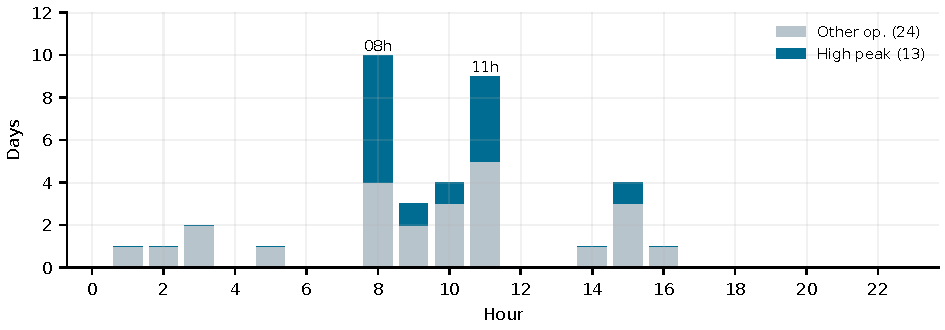
\includegraphics[width=\linewidth]{peak_hours.pdf}
\caption{개발 구간 가동일 37일의 첫 피크 시각 분포. 짙은 색은 고피크일 13일, 옅은 색은 그 밖의 가동일 24일이다(그림 속 범례는 영어: High peak, Other op.).}\label{fig:ch1-peakhours}
\end{figure}

\hwpsection{1.3 데이터 진단 및 전처리}

전처리에서는 기록 오류, 중복, 정보 누수를 통제하였다. 높은 전력값은 피크 분석에 필요한 관측값이므로 크기만을 기준으로 제거하거나 상한을 두지 않았다.
\begin{hwplist}
\item 시계열 정렬: 시간별 행의 전력 4개 열을 15분 슬롯으로 펼쳐 단일 시계열로 만들고 각 슬롯에 시작 시각을 부여하였다. 시간별 생산량과 기상은 그 시간의 네 슬롯에 같은 값으로 연결하되, 일 총생산량은 원래 시간별 값을 합산하여 중복 집계를 막았다.
\item 시각 오류: 7월 13일과 15일의 48개 행에서 기록된 시각 열이 행 순서와 맞지 않았다. 두 날의 전력과 생산량을 결측 처리하고 오류 표지를 유지하여 학습과 평가에서 제외하였다. 자료 정렬에는 행 순서를 썼으며, 이를 실제 시각의 복원으로 보지는 않았다.
\item 전력 결측: 전력 0값 74개(8월 28일 26개, 8월 29일 46개, 9월 8일 2개)를 계측 손실로 보고 결측 처리하였다. 피크 왜곡을 막기 위해 목표 전력은 보간하지 않았다. 슬롯 오차는 관측된 슬롯만으로 계산하고, 일 피크 평가는 결측이 4슬롯 이하인 날로 제한하였다.
\item 중복 제거: 하루 96개 전력값이 소수점까지 같은 날을 한 묶음으로 보고 한 날만 원본으로 남겨 115일을 완전 복사일로 표시하였다. 원본은 시간순 첫 날로 하되, 첫 날이 생산 없이 40 kW를 넘는 슬롯을 48개 이상 가지면 생산이 있는 날을 원본으로 삼았다. 같은 복사쌍의 기온과 습도 시계열은 115쌍 모두 서로 달라, 전력 곡선만 복사해 넣은 증강 자료로 판단하였다. 나머지 날 가운데 40 kW를 넘는 슬롯이 다른 날의 같은 슬롯과 20개 이상 일치한 7일은 편집 복사일로 분류하였다. 복사일 122일(257일의 47\%)의 전력은 결측 처리하여 학습, 평가, 과거 전력 참조에서 제외하였다.
\item 정보 누수 변수: 공장인원은 생산량을 한 시간 안 전력 네 값의 합으로 나눈 값과 일치하였고(유효 6,151행, 최대 절대오차 $5\times10^{-9}$), 평균은 전력 네 값의 평균을 반올림한 값과 6,168행 모두 일치하였다. 예측 대상이 계산에 들어 있는 두 열을 입력에서 제외하였으며, 공장인원을 실제 작업자 수로 해석하지 않았다.
\item 기상정보: 풍속 결측 3개 시간은 선형보간하고, 누적 강수량은 날짜 경계를 포함한 연속 차분으로 증분화하였다. 음의 차분은 누적값이 초기화된 것으로 보아 현재값을 사용하였다. 강수량 결측 1개 시간은 증분을 0으로 두고 직전 유효 누적값을 유지하였다.
\item 파생변수: 생산량에서 생산 여부, 하루 생산시간, 일 총생산량, 가동유형을 만들었다. C-BAT에는 생산 여부와 정규화한 로그 생산량을 구분하여 입력하였다. 요일, 월, 평일·토·일은 날짜에서 만들고 공휴일은 별도 목록으로 관리하였다. 정규화 기준과 전력 기본 수준은 학습 기간에서만 산출하였다.
\end{hwplist}
\hwpnote{전력 0값의 원인이 실제 정전인지 계측 누락인지는 확인되지 않았다. 결측이 적은 날에도 관측되지 않은 슬롯에서 일 피크가 발생했을 가능성은 남아 있다.}

\hwpsection{1.4 예측 시점의 정보 사용 범위와 검증 설계}

매일 00:00 시점에 당일 96슬롯의 전력을 예측하도록 설정하였다. 입력은 당일의 시간별 생산계획, 사전에 알 수 있는 달력 정보, 예측일 이전에 관측된 전력으로 한정하였다. 모든 모형은 예측일과 그 이후의 전력을 가린 자료로 예측하므로 당일과 미래의 전력값은 입력에 들어가지 않는다.

제공된 자료에는 생산 실적만 있고 사전 생산계획은 없다. 생산 실적을 전날 확정된 생산계획으로 간주하였으므로, 이 보고서의 모든 성능은 시간별 생산계획을 미리 안다는 가정에서 나온 값이다. 현장 적용 시에는 실제 계획 자료를 연결하고 계획과 실적의 차이가 미치는 영향을 확인해야 하며, 이 영향은 3장의 입력 오차 실험에서 살핀다.

복사일이 섞인 자료에서 날짜를 무작위로 나누면 시험일의 사본이 학습에 들어간다. 이를 확인하기 위해 9월 이전에 관측된 241일을 날짜 단위 무작위 5-fold와 LOEO(leave-one-event-out)로 비교하였다. LOEO는 같은 전력 곡선을 공유하는 날의 묶음(복사 사건)을 함께 제외하며, 사건은 126개(복사군 45개, 단독일 81개)이다. M2의 MAE는 무작위 분할에서 14.91 kW, LOEO에서 16.64 kW로 차이는 $-1.73$ kW이고 95\% 신뢰구간은 0을 포함하지 않는다(표~\ref{tab:ch1-leak}). 기존 BAT는 두 분할에서 거의 같았다. 무작위 분할은 M2를 약 10\% 낙관적으로 보이게 하는 누수를 만들었다.

\begin{table}[htbp]
\centering
\hwptablefont
\caption{복사일을 포함한 자료의 누수 진단(MAE, kW, 관측 241일). 차이는 무작위 5-fold에서 LOEO를 뺀 값이다.}\label{tab:ch1-leak}
\begin{tabular}{lrrr}
\toprule
모형 & 무작위 5-fold & LOEO & 차이 [95\% 신뢰구간] \\
\midrule
M2 (LightGBM 기본) & 14.91 & 16.64 & $-1.73$ [$-3.63$, $-0.04$] \\
기존 BAT & 16.37 & 16.32 & $+0.05$ [$-0.22$, $+0.42$] \\
\bottomrule
\end{tabular}
\end{table}
\hwpnote{신뢰구간은 날짜 단위 짝지은 부트스트랩(2,000회)으로 구하였다. 진단 실행은 시간을 줄이려 기존 BAT를 1,000회 표집(초기 500회 제외), M2를 100회 부스팅으로 줄인 설정이며, 누수의 정도를 보는 값이지 전방 예측 성능의 추정치가 아니다.}

이 결과에 따라 모든 모형 비교는 복사일을 목표에서 뺀 시간순 분할로 하였다. 개발 구간의 검증 구간 f1--f4는 2021년 7월 7일부터 8월 31일까지 14일씩 네 개(f1 7월 7--20일, f2 7월 21일--8월 3일, f3 8월 4--17일, f4 8월 18--31일)이며, 각 검증 구간의 모형은 그 이전 자료만으로 학습한다. 검증 첫날의 전날은 간격일로 두어 목표에서 빼고 첫 검증일의 입력으로만 쓴다. 검증 구간과 같은 복사 사건에 속한 학습일은 제거(purge)하는 규칙을 두었으나 실제로 해당하는 날은 없었다. 학습 기간에는 복사일이 많아(표~\ref{tab:ch1-copies}), f1의 학습 기간은 달력상 186일이지만 복사일 121일(65\%)을 빼면 65일이다.

\begin{table}[htbp]
\centering
\hwptablefont
\caption{검증 구간별 학습 기간의 달력일과 복사일(일).}\label{tab:ch1-copies}
\begin{tabular}{lrrr}
\toprule
검증 구간 & 학습 달력일 & 복사일 & 복사 제외 \\
\midrule
f1 & 186 & 121 & 65 \\
f2 & 200 & 121 & 79 \\
f3 & 214 & 122 & 92 \\
f4 & 228 & 122 & 106 \\
9월 시험 & 242 & 122 & 120 \\
\bottomrule
\end{tabular}
\end{table}

개발 구간 56일 가운데 시각 오류일 2일(7월 13일, 15일)과 복사일 1일(7월 30일)은 목표가 없어 채점에서 빠지므로, 유효하게 채점되는 날은 53일(5,016슬롯)이다. 이 중 8월 28일과 29일은 결측이 5슬롯 이상이어서 일 피크 평가일은 51일이다.

9월 1--14일은 최종 평가를 위한 9월 시험 구간으로 봉인하였다. 기본 로더가 이 구간의 목표와 입력을 모두 가리며, 이전 개발 단계에서 한 번 열린 적이 있어 완전한 미사용 구간은 아니다. C-BAT는 개발 구간에서 확정하여 동결한 뒤 9월에 적용하였고, 9월 결과로 구조나 하이퍼파라미터를 고르지 않았다. 주 성능은 개발 구간과 9월 시험 구간을 합친 67일·6,358슬롯(피크 평가일 65일)의 시간순 평가(합산 평가)로 제시하며, 합산 평가의 정의는 2.2절에서 다룬다. 모델 선택, 절제, 오류분석은 개발 구간에서, 9월 단독 결과는 보조로 사용하였다.

\hwpchapter{2}{AI 예측모델 개발 및 성능평가}{40}

제안모형 C-BAT는 시간별 생산계획을 15분 슬롯 전력으로 옮기는 조건부 베이지안 전달모형이다. 이 장은 C-BAT의 수식, 기호, 모수와 추정 방법(2.1절), 비교모델과 공통 평가조건(2.2절), 모델별 성능과 최종모델 선정 근거(2.3절)를 차례로 제시한다. 주 성능은 개발 구간과 9월 시험 구간을 합친 합산 평가(67일, 6,358슬롯, 피크 평가일 65일)로 보고하고, 모델 선택과 절제 비교는 개발 구간(53일, 5,016슬롯, 피크 평가일 51일)에서 수행하였다.

\hwpsection{2.1 제안모형 C-BAT의 구조와 추정}

예측 과제는 예측일 $d$의 00:00에 그날 96개 슬롯의 전력 $y_{d,t}$($t=1,\dots,96$)를 한꺼번에 내는 것이다. 이 시점에 쓰는 정보는 그날의 시간별 생산계획 $q_{d,h}$($h=0,\dots,23$), 가동 여부와 날짜유형(평일·토요일·일요일), 그리고 $d-1$일까지 관측된 전력뿐이며, 예측일 당일의 전력은 한 슬롯도 쓰지 않는다(1.4절). C-BAT는 점예측 하나가 아니라 하루 96슬롯 전력 경로의 예측분포를 내고, 이 분포에서 다음 세 산출물을 얻는다.
\begin{hwplist}
\item 슬롯 예측: 슬롯별 분위수(5\%에서 95\%까지 5\% 간격)와 점예측(중앙값).
\item 일 피크 분포: 일 피크 $M_d=\max_t y_{d,t}$의 예측분포와 그 중앙값.
\item 피크 초과확률: 학습 기간에서 정한 피크 기준 $C\in\{C_{50},C_{75},C_{90}\}$에 대한 $P(M_d>C)$.
\end{hwplist}
슬롯마다 따로 만든 분위수로는 하루 최댓값의 분포를 얻을 수 없으므로, 하루 곡선 전체를 한꺼번에 표집하는 구조로 설계하였다. 그림~\ref{fig:ch2-structure}은 입력에서 산출물까지의 흐름이다.

\begin{figure}[htbp]
\centering
\begin{tikzpicture}[font=\footnotesize, >=latex,
  box/.style={draw, rounded corners=2pt, align=center, inner sep=3pt, minimum height=9mm},
  inp/.style={box, fill=gray!8, text width=3.0cm},
  mid/.style={box, fill=blue!6, text width=3.4cm},
  pth/.style={box, fill=blue!12, text width=3.6cm},
  outp/.style={box, fill=green!7, text width=3.0cm}]
\node[inp] (q) at (0,1.5) {당일 시간별 생산계획\\$q_{d,h}$, 가동유형 $k$};
\node[inp] (r) at (0,0) {기준일 곡선 $r_{d,t}$\\($d-1$일까지의 전력)};
\node[inp] (g) at (0,-1.5) {잡음 상태 $g$\\(비가동 / 가동)};
\node[mid] (m) at (4.3,0.75) {평균 곡선 $m_{d,t}$\\기본곡선 $\mu_{k,t}$ + 기준일 항\\+ 생산 전달항};
\node[mid] (n) at (4.3,-1.5) {상태별 잡음\\날짜 효과 $u_d$ + AR(1) $e_{d,t}$};
\node[pth] (p) at (8.5,-0.4) {사후 경로 3,000개\\$\tilde y^{(s)}_{d,t}=s_y(m+u+e)$\\(음수는 0으로 절단)};
\node[outp] (o1) at (12.6,1.1) {슬롯 분위수\\점예측(중앙값)};
\node[outp] (o2) at (12.6,-0.4) {일 피크 분포\\$\tilde M^{(s)}_d=\max_t \tilde y^{(s)}_{d,t}$};
\node[outp] (o3) at (12.6,-1.9) {피크 초과확률\\$P(M_d>C)$};
\node[box, fill=orange!8, text width=6.0cm] (e) at (3.3,-3.3) {학습 기간 추정(반감기 30일 시간 가중)\\Gibbs--Metropolis 6,000회, 앞 3,000회 제외\\$\Rightarrow$ 사후표본 $\Theta^{(s)}$, $s=1,\dots,3{,}000$};
\draw[->] (q) -- (m);
\draw[->] (r) -- (m);
\draw[->] (g) -- (n);
\draw[->] (m) -- (p);
\draw[->] (n) -- (p);
\draw[->] (p) -- (o1);
\draw[->] (p) -- (o2);
\draw[->] (p) -- (o3);
\draw[->] (e.east) -| node[pos=0.25, above] {표본마다 경로 1개} (p.south);
\end{tikzpicture}
\caption{C-BAT의 구조. 생산계획과 기준일 곡선이 평균 곡선을 정하고, 가동 상태별 잡음을 더한 사후 경로 묶음에서 세 산출물을 모두 계산한다.}\label{fig:ch2-structure}
\end{figure}

학습 기간의 관측 전력 표준편차 $s_y$로 전력을 나누어 $z_{d,t}=y_{d,t}/s_y$로 변환하였다(평균은 빼지 않는다). 표준화 전력은 평균 곡선 세 항과 변동 두 항의 합이다.
\begin{equation}
z_{d,t} \;=\; \underbrace{\mu_{k,t}}_{\text{기본곡선}}
\;+\; \underbrace{\gamma_k\, r_{d,t}}_{\text{기준일}}
\;+\; \underbrace{\sum_{c\in\{\mathrm{on},\,\log\}} w_{c,k} \sum_{h=0}^{23} \alpha_{t,h}\, x_c(q_{d,h})}_{\text{생산 전달항}}
\;+\; \underbrace{u_d}_{\text{날짜 효과}}
\;+\; \underbrace{e_{d,t}}_{\text{슬롯 잡음}}
\label{eq:ch2-cbat}
\end{equation}
$k$는 예측일 $d$의 가동유형이다. 앞의 세 항은 생산계획과 최근 운전 상태가 정하는 평균 곡선 $m_{d,t}$이고 뒤의 두 항은 그 주변의 변동이다. 이름의 C(conditional)는 변동의 크기와 지속성을 가동 상태별로 따로 두는 데서 붙였다. 예측할 때에는 식의 오른쪽 전체에 $s_y$를 곱해 kW로 되돌린다. $s_y$와 생산량 정규화 기준 $q_{\max}$는 해당 학습 기간에서만 계산하며, 검증일이나 9월 자료로 갱신하지 않는다. 사용한 기호는 표~\ref{tab:ch2-notation}에 정리하였다.

\begin{table}[htbp]
\centering
\hwptablefont
\caption{C-BAT의 주요 기호.}\label{tab:ch2-notation}
\begin{tabular}{L{4.4cm}L{11.2cm}}
\toprule
기호 & 의미 \\
\midrule
$d$, $t=1,\dots,96$, $h=0,\dots,23$ & 예측일, 15분 슬롯, 생산계획의 시각 \\
$y_{d,t}$, $s_y$, $z_{d,t}=y_{d,t}/s_y$ & 슬롯 전력(kW), 학습 기간 관측 전력의 표준편차, 표준화 전력 \\
$q_{d,h}$, $q_{\max}$ & 시간별 생산계획량, 학습 기간의 시간별 최대 생산량 \\
$k\in\{0,1,2,3\}$ & 가동유형(계획 생산시간 0시간 / 1--12시간 / 13--19시간 / 20시간 이상) \\
$g\in\{\text{비가동},\text{가동}\}$ & 잡음 상태($k=0$이면 비가동, $k\ge1$이면 가동) \\
$\mu_{k,t}$, $\tau_k$ & 가동유형별 기본곡선(표준화 단위)과 그 평활 분산 \\
$r_{d,t}$, $\gamma_k$ & 표준화한 기준일 곡선과 그 계수 \\
$x_c(q)$, $c\in\{\mathrm{on},\log\}$ & 생산 채널(생산 여부, 정규화 로그 생산량) \\
$w_{c,k}=e^{\omega_{c,k}}$ & 채널·가동유형별 생산 이득(양수), $\omega_{c,k}$는 그 로그 \\
$\alpha_{t,h}$, $\Delta_{t,h}$ & 시간 계획을 슬롯으로 옮기는 커널 가중치, 슬롯 $t$와 시각 $h$의 중앙 시각 차이(시간) \\
$\sigma$, $\beta$, $\ell$ & 커널의 척도, 형상, 시차(코드의 $c$) \\
$u_d$, $\sigma_{u,g}$ & 날짜 효과와 그 표준편차 \\
$e_{d,t}$, $\rho_g$, $\sigma_{\eta,g}$ & 슬롯 AR(1) 잡음, 자기상관, 혁신 표준편차 \\
$\kappa_d$, $\mathcal T$, $\mathcal O_d$ & 반감기 시간 가중치, 유효 학습일 집합, $d$일의 관측 슬롯 집합 \\
$m_{d,t}$, $\tilde y^{(s)}_{d,t}$, $S$ & 평균 곡선(식~\ref{eq:ch2-cbat}의 앞 세 항), 사후표본 $s$의 예측 경로, 경로 수($S=3{,}000$) \\
$M_d$, $\tilde M^{(s)}_d$ & 일 피크 $\max_t y_{d,t}$, 경로 $s$의 하루 최댓값 \\
$C_{50}$, $C_{75}$, $C_{90}$ & 학습 기간 가동일 일 피크의 50·75·90\% 분위수(피크 기준) \\
\bottomrule
\end{tabular}
\end{table}

가동유형 $k$는 그날 계획에서 생산량이 양수인 시간 수로 정하므로 00:00에 알 수 있다. 기본곡선, 기준일 계수, 생산 이득은 가동유형마다 따로 두었다. 운전 시간이 다른 날은 하루 곡선의 모양 자체가 다르기 때문이다. 기본곡선 $\mu_{k,t}$는 가동유형별 하루 평균 모양을 맡으며 96개 값에 순환 2차 확률보행(RW2) 사전분포를 두었다. 인접 슬롯의 이차 차분 $\mu_{k,t+1}-2\mu_{k,t}+\mu_{k,t-1}$에 벌점을 주고 슬롯 96과 슬롯 1을 이어 자정 전후도 매끄럽게 하였다. 평활 분산 $\tau_k$도 유형마다 추정하므로 자료가 적은 유형의 곡선은 더 매끄럽게 수축된다.

기준일 곡선 $r_{d,t}$는 최근 공장 상태를 평균에 반영한다. 기준일은 예측일 이전 28일 안에서 가동 여부와 날짜유형이 모두 같은 완전 관측일(96슬롯 모두 관측) 가운데 가장 최근 날이며, 그날 전력을 $s_y$로 나누어 $r_{d,t}$를 만든다. 28일 안에 그런 날이 없으면 전체 과거에서 가동 여부만 같은 가장 최근 완전 관측일을, 그것도 없으면 학습 기간의 해당 가동유형 평균 곡선을 쓴다. 계수 $\gamma_k$는 기준일 곡선을 얼마나 따를지 정한다. 기본곡선이 학습 기간 전체의 평균 모양을 맡는다면 기준일 항은 계절에 따라 움직이는 최근 수준을 따라간다.

생산 전달항은 시간별 생산계획을 슬롯 전력의 증가분으로 옮긴다. 계획량은 두 채널로 바꾼다.
\begin{equation}
x_{\mathrm{on}}(q)=\mathbf 1[q>0],\qquad
x_{\log}(q)=\frac{\log(1+q)}{\log(1+q_{\max})}.
\label{eq:ch2-channels}
\end{equation}
첫 채널은 라인이 도는지를, 둘째 채널은 생산량의 크기를 나타낸다. 이득은 $w_{c,k}=\exp(\omega_{c,k})$로 두어 양수로 제약하였다. 따라서 가동유형과 기준일이 같은 상태에서 생산량만 늘리면 전달항은 줄지 않는다. 다만 생산시간이 바뀌어 가동유형이 달라지면 기본곡선과 계수도 바뀌므로 전체 예측의 단조성까지 보장하지는 않는다. 비가동일($k=0$)에는 생산이 없으므로 전달항을 두지 않는다($w_{c,0}=0$).

시간 계획을 슬롯으로 옮기는 가중치 $\alpha_{t,h}$는 다음의 고정 sparsemax 커널이다.
\begin{equation}
\alpha_{t,\cdot} = \operatorname{sparsemax}\!\left(-\frac{\lvert \Delta_{t,h} - \ell\rvert^{\beta}}{\sigma}\right)_{h=0,\dots,23},
\qquad \Delta_{t,h}=\frac{t-4h-2.5}{4},
\qquad (\sigma,\beta,\ell)=(1.5,\ 2,\ 0).
\label{eq:ch2-kernel}
\end{equation}
$\Delta_{t,h}$는 슬롯 $t$의 중앙 시각과 시각 $h$의 중앙 시각의 차이(시간 단위)다. sparsemax는 점수 벡터 $\boldsymbol v$를 확률 단체에 유클리드 사영하는 변환으로 $\operatorname{sparsemax}(\boldsymbol v)_h=\max\{v_h-\tau(\boldsymbol v),0\}$이며, $\tau(\boldsymbol v)$는 가중치 합을 1로 맞추는 문턱값이다. 그래서 먼 시각의 가중치는 정확히 0이 된다. 척도 $\sigma=1.5$, 형상 $\beta=2$, 시차 $\ell=0$시간은 사전분포의 중심값에 고정한 값이며 검증 점수를 보고 고르지 않았다($\sigma$는 점수 함수의 척도이고 잡음의 표준편차가 아니다). 이 값에서 첫 슬롯과 마지막 슬롯은 한 시각, 나머지 94개 슬롯은 인접한 두 시각에만 가중치를 둔다. 예컨대 00:30--00:45 슬롯은 0시 계획에 0.75, 1시 계획에 0.25를 두고, 00:45--01:00 슬롯은 0.58과 0.42를 둔다. 즉 각 슬롯의 전달 입력은 가까운 두 시각 계획의 가중 평균이며 시차는 없다.

날짜 효과와 슬롯 잡음은 잡음 상태 $g$마다 따로 두었다.
\begin{equation}
u_d \sim \mathcal N\big(0,\ \sigma^2_{u,g}\big),
\qquad
e_{d,t} = \rho_g\, e_{d,t-1} + \eta_{d,t},\quad \eta_{d,t}\sim \mathcal N\big(0,\ \sigma^2_{\eta,g}\big).
\label{eq:ch2-noise}
\end{equation}
날짜 효과 $u_d$는 하루 전체를 함께 올리거나 내리는 변동이고, $e_{d,t}$는 슬롯 사이에 이어지는 1차 자기회귀 잡음이다. 하루 첫 슬롯은 정상분포 $\mathcal N\big(0,\sigma^2_{\eta,g}/(1-\rho_g^2)\big)$에서 시작한다. 조용한 비가동일과 생산 부하가 오르내리는 가동일은 변동의 크기와 지속 시간이 다르다. 두 상태가 같은 잡음을 공유하면 비가동일 경로가 가동일 수준으로 흔들려 비가동일의 일 피크가 과대평가되므로 잡음을 상태별로 나누었다.

우도는 관측된 슬롯만으로 계산하고 결측 슬롯은 대체하지 않는다. 같은 날 관측 슬롯 $t$와 바로 앞 관측 슬롯 $t-s$ 사이에 $s-1$개 슬롯이 비어 있으면 AR(1)의 $s$단계 전이분포를 쓴다.
\begin{equation}
e_{d,t} \mid e_{d,t-s} \;\sim\; \mathcal N\!\left(\rho_g^{\,s}\, e_{d,t-s},\ \ \sigma^2_{\eta,g}\,\frac{1-\rho_g^{\,2s}}{1-\rho_g^{\,2}}\right).
\label{eq:ch2-gap}
\end{equation}
그날의 첫 관측 슬롯은 정상분포에서 나온다고 둔다. 결측이 없는 날에는 식~\eqref{eq:ch2-noise}의 우도와 같아지고, 결측 구간이 잡음 추정을 왜곡하지 않는다.

모수는 시간 가중 우도를 쓰는 Gibbs--Metropolis 표집으로 추정하였다. 날짜 $d$의 관측은 우도에서 다음 가중치를 받는다.
\begin{equation}
\kappa_d = 2^{-(d_{\max}-d)/30},\qquad
\pi(\Theta,\boldsymbol u\mid\boldsymbol z)
\;\propto\;\pi(\Theta)\prod_{d\in\mathcal T}
p(u_d\mid\Theta)\,
p(\boldsymbol z_{d,\mathcal O_d}\mid\Theta,u_d)^{\kappa_d}.
\label{eq:ch2-weight}
\end{equation}
$d_{\max}$는 전력이 하나 이상 관측된 학습일의 마지막 날이며, 30일 전 자료의 가중치는 절반이다. $\Theta$는 날짜 효과를 제외한 모수다. 가중치는 AR(1) 우도 전체(정규화항 포함)에 지수로 적용하고 날짜 효과의 사전분포에는 곱하지 않는다. 공장 전력 수준이 계절에 따라 움직이므로 모든 날을 같은 무게로 두면 최근 수준을 따라가지 못하기 때문이다. 한 번의 반복은 다음 순서로 진행한다.
\begin{hwplist}
\item 백색화: 현재 $\rho_g$와 결측 간격 $s$로 AR(1) 백색화 계수($\phi=\rho_g^s$, 첫 관측은 $\phi=0$)를 계산한다.
\item 생산 이득: 가동유형 $k=1,2,3$마다 두 로그 이득 $\omega_{\cdot,k}$에 보폭 0.5의 정규 랜덤워크를 제안하고, 평균 모수 $(\boldsymbol\mu_k,\gamma_k)$를 적분한 주변우도와 사전분포로 Metropolis 채택 여부를 정한다. 학습 자료에 그 유형이 없으면 사전분포에서 뽑는다.
\item 평균 블록: 가동유형마다 기본곡선 96개와 기준일 계수를 합친 97차원 벡터를 결합 정규 조건부분포에서 Cholesky 분해로 한꺼번에 뽑는다(식~\ref{eq:ch2-mean-block}).
\item 분산과 날짜 효과: 평활 분산 $\tau_k$를 역감마 조건부분포 $\mathrm{IG}\big(49,\ 0.01+\tfrac12\boldsymbol\mu_k^{\mathsf T}\mathbf R_\epsilon\boldsymbol\mu_k\big)$에서, 날짜 효과 $u_d$를 사전분포와 그날 백색화 잔차의 가중 우도를 결합한 켤레 정규분포에서 뽑는다.
\item 잡음 모수: 잡음 상태마다 $\rho_g$를 보폭 0.04의 랜덤워크 Metropolis로 갱신하고($[0,\,0.98)$ 밖의 제안은 기각), $\sigma^2_{\eta,g}$와 $\sigma^2_{u,g}$를 켤레 역감마 조건부분포에서 뽑는다. $\sigma^2_{\eta,g}$의 모양 모수에는 관측 수 대신 가중치 합의 절반을 더한다.
\end{hwplist}
평균 블록의 조건부분포는 백색화한 설계행렬 $\mathbf H_k$, 백색화 목표 $\boldsymbol b_k$(표준화 전력에서 전달항과 날짜 효과를 뺀 값), 관측 정밀도 $\mathbf W_k=\operatorname{diag}(\kappa_{d(i)}/\sigma^2_{\eta,g})$로 다음과 같다.
\begin{equation}
\begin{split}
\begin{pmatrix}\boldsymbol\mu_k\\\gamma_k\end{pmatrix}\Bigm|\text{나머지}
&\sim\mathcal N\!\left(\mathbf A_k^{-1}\mathbf H_k^{\mathsf T}\mathbf W_k\boldsymbol b_k,\ \mathbf A_k^{-1}\right),\\
\mathbf A_k &= \mathbf H_k^{\mathsf T}\mathbf W_k\mathbf H_k
+\operatorname{blockdiag}\!\left(\frac{\mathbf R_\epsilon}{\tau_k},\ \frac1{25}\right),\qquad
\mathbf R_\epsilon=\mathbf R+10^{-4}\mathbf I.
\end{split}
\label{eq:ch2-mean-block}
\end{equation}
$\mathbf R$은 순환 RW2 정밀도 행렬이다. 표집은 6,000회 반복하고 앞 3,000회를 버려 남은 3,000개 사후표본을 예측 경로 3,000개로 쓴다. 초기값은 $\omega_{c,k}=\log0.3$, $\mu_{k,\cdot}$는 가동유형별 학습 평균 곡선, $\gamma_k=0$, $\rho_g=0.5$이다. 수렴은 시드 0--2의 세 사슬로 기본 split-$\hat R$을 계산해 점검하였다. 상수 모수를 뺀 22개 모수의 최댓값은 1.029로, 개발 구간 네 검증 구간의 모든 적합 단계에서 기준 1.05를 넘은 모수가 없었다. 이 진단은 순위 정규화 $\hat R$이나 꼬리 유효표본 수 진단이 아니므로 수렴의 충분조건은 아니다. 모수의 고정값과 사전분포는 표~\ref{tab:ch2-params}에 모았다.

{\hwptablefont
\setlength{\tabcolsep}{3pt}
\begin{longtable}{L{1.8cm}L{2.8cm}L{1.6cm}L{4.0cm}L{5.2cm}}
\caption{C-BAT의 모수. IG는 역감마(모양, 척도)이며 값은 표준화 단위이다.}\label{tab:ch2-params}\\
\toprule
기호 & 의미 & 고정/추정 & 값 또는 사전분포 & 근거·코드 \\
\midrule
\endfirsthead
\caption[]{C-BAT의 모수(계속).}\\
\toprule
기호 & 의미 & 고정/추정 & 값 또는 사전분포 & 근거·코드 \\
\midrule
\endhead
\midrule
\multicolumn{5}{r}{\footnotesize 다음 쪽에 계속}\\
\endfoot
\bottomrule
\endlastfoot
$s_y$, $q_{\max}$ & 전력 척도, 생산량 정규화 기준 & 학습 자료로 계산 & 학습 기간 관측 전력의 표준편차, 시간별 최대 생산량 & 검증 구간마다 다시 계산. \texttt{fit\_conditional} \\
$\mu_{k,\cdot}$ & 가동유형별 기본곡선 & 추정 & $\mathcal N\big(0,\ \tau_k\mathbf R_\epsilon^{-1}\big)$, 순환 RW2 & 인접 슬롯과 자정 전후를 매끄럽게 연결. \texttt{bat.\_rw2} \\
$\tau_k$ & 평활 분산 & 추정 & $\mathrm{IG}(1,\ 0.01)$ & 유형별 평활 강도를 자료로 결정 \\
$\gamma_k$ & 기준일 계수 & 추정 & $\mathcal N(0,\ 5^2)$ & 약한 정보 사전분포 \\
$\omega_{c,k}$ ($k=1,2,3$) & 로그 생산 이득 & 추정 & $\mathcal N(\log0.3,\ 1.5^2)$, 제안 보폭 0.5 & $w=e^{\omega}>0$이면 생산이 늘 때 전달항이 줄지 않음. \texttt{bat.PRIOR\_MU}, \texttt{PRIOR\_SD} \\
$w_{c,0}$ & 비가동일 이득 & 고정 & 0 & 비가동일에는 생산이 없음 \\
$\sigma$, $\beta$, $\ell$ & 커널 척도·형상·시차 & 고정 & 1.5, 2, 0시간 & 사전분포 중심값. 학습형 커널은 수렴 기준 미달(최대 $\hat R$ 1.308, 2.3절). \texttt{fixed\_attention=True} \\
$\sigma^2_{u,g}$ & 날짜 효과 분산 & 추정 & $\mathrm{IG}(2,\ 0.01)$ & 잡음 상태별 \\
$\sigma^2_{\eta,g}$ & 혁신 분산 & 추정 & $\mathrm{IG}(2,\ 0.01)$ & 잡음 상태별 \\
$\rho_g$ & AR(1) 자기상관 & 추정 & $\mathrm U[0,\ 0.98)$, 제안 보폭 0.04 & 정상성 보장 \\
반감기 & 시간 가중 $\kappa_d$ & 고정 & 30일 & 최근 전력 수준 추종. \texttt{half\_life=30} \\
기준일 규칙 & $r_{d,t}$의 선택 & 고정 & 28일 이내, 가동 여부·날짜유형 일치 & B0$'$ 규칙과 같음. \texttt{ref="op"}, \texttt{b0p\_ref} \\
표집 & 반복·제외 횟수 & 고정 & 6,000회, 앞 3,000회 제외 & 최종 실행 인자(\texttt{main.py}). 코드 기본값은 2,000회·1,000회 \\
$C_{50}$, $C_{75}$, $C_{90}$ & 피크 기준 & 학습 자료로 계산 & 가동일·결측 4슬롯 이하 일 피크의 50·75·90\% 분위수 & 검증 구간마다 다시 계산. \texttt{evaluate.py}의 \texttt{thresholds} \\
\end{longtable}}
\hwpnote{코드는 \path{gmst/conditional_bat.py}(적합·예측), \path{gmst/bat.py}(커널, 채널, 사전분포 중심값, 기준일), \path{gmst/conditional_ar.py}(결측 간격 백색화)에 있다.}

추정된 잡음 모수는 상태를 나눈 이유를 보여 준다(그림~\ref{fig:ch2-noise}). 개발 구간 네 검증 구간과 시드 0--2의 사후표본을 모으면, 슬롯 혁신 표준편차의 중앙값은 비가동 1.60 kW, 가동 8.37 kW로 가동 상태가 약 다섯 배 크고, 자기상관 $\rho_g$의 중앙값은 각각 0.78과 0.91이다. 날짜 효과 표준편차의 중앙값은 2.73 kW와 3.64 kW로 차이가 작다.

\begin{figure}[htbp]
\centering
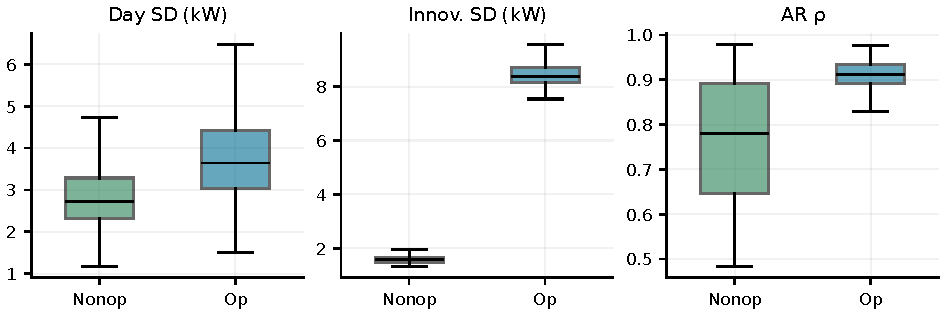
\includegraphics[width=\linewidth]{noise_state.pdf}
\caption{잡음 상태별 사후분포(개발 구간 f1--f4, 시드 0--2의 사후표본 합산). 왼쪽부터 날짜 효과 표준편차(Day SD), 슬롯 혁신 표준편차(Innov.\ SD), AR(1) 자기상관($\rho$)이며 Nonop은 비가동, Op은 가동 상태이다. 상자는 25·50·75\% 분위수, 수염은 사분위범위의 1.5배이다.}\label{fig:ch2-noise}
\end{figure}

예측분포는 사후표본마다 하루 경로 하나를 만들어 얻는다. 사후표본 $s=1,\dots,S$의 모수로 예측일 계획에서 평균 곡선 $m^{(s)}_{d,t}$를 계산하고, 새 날짜 효과와 AR(1) 잡음을 더한다.
\begin{equation}
\tilde y^{(s)}_{d,t} = \max\!\Big\{0,\ s_y\big(m^{(s)}_{d,t} + u^{(s)}_d + e^{(s)}_{d,t}\big)\Big\},
\qquad u^{(s)}_d\sim\mathcal N\big(0,\sigma^{2(s)}_{u,g}\big),\quad
e^{(s)}_{d,t}=\rho^{(s)}_g e^{(s)}_{d,t-1}+\eta^{(s)}_{d,t}.
\label{eq:ch2-path}
\end{equation}
잡음 상태 $g$는 그날 계획의 가동유형으로 정하고, 전력은 음수가 될 수 없으므로 0에서 자른다. 난수 시드는 예측 날짜로 정해 같은 입력에서 같은 경로가 나온다. 점예측은 슬롯별 경로 중앙값이고, 분위수는 경로의 5--95\% 분위수(q05--q95)이다. 일 피크의 분포는 경로마다 구한 최댓값 $\tilde M^{(s)}_d=\max_t \tilde y^{(s)}_{d,t}$의 분포이며 피크 점예측은 그 중앙값이다. 이 값은 슬롯별 중앙값 곡선의 최댓값과 일반적으로 다르다. 피크 초과확률은 최댓값이 기준을 넘는 경로의 비율이다.
\begin{equation}
\hat P(M_d > C) = \frac1S\sum_{s=1}^{S}\mathbf 1\big[\tilde M^{(s)}_d > C\big],
\qquad C\in\{C_{50},C_{75},C_{90}\}.
\label{eq:ch2-risk}
\end{equation}
피크 기준 $C_{50},C_{75},C_{90}$은 학습 기간 가동일 가운데 결측 슬롯이 4개 이하인 날의 관측 일 피크의 50·75·90\% 분위수이며 학습 기간이 바뀌면 다시 계산한다. 발행 시에는 96슬롯 전체에서 경로 최댓값을 구하고, 채점 시에는 관측 슬롯에 대응하는 경로만으로 최댓값을 다시 구해 관측 피크와 비교한다. 이 마스크는 사후 채점 규칙이며 발행 예측에 미래의 결측 여부를 넣는 것이 아니다. 발행하는 초과확률은 식~\eqref{eq:ch2-risk}의 보정 전 경로 확률이며, 짧은 보정 기간의 Platt 보정을 쓰지 않은 이유는 3.3절에서 설명한다.

\hwpsection{2.2 비교모델 및 평가조건}

C-BAT의 구성 요소별 효과와 범용 기계학습 대비 성능을 확인하기 위해 다섯 비교모델을 두었다(표~\ref{tab:ch2-models}).

\begin{table}[htbp]
\centering
\hwptablefont
\setlength{\tabcolsep}{3pt}
\caption{비교모델의 입력, 구조, 역할.}\label{tab:ch2-models}
\begin{tabular}{L{2.3cm}L{4.4cm}L{5.3cm}L{3.4cm}}
\toprule
모델 & 입력 & 구조와 출력 & 역할 \\
\midrule
B0 & 7일 전 같은 슬롯의 전력. 그 슬롯이 결측이면 B0$'$ 기준일(28일 이내 가동 여부·날짜유형 일치 최근 완전 관측일)의 값 & 과거 곡선 복사. 점예측만 냄 & 생산계획을 쓰지 않는 최소 기준선 \\
B0\_kind & 28일 이내에서 가동유형과 날짜유형이 같은 가장 최근 완전 관측일. 없으면 같은 가동유형, 그다음 가장 최근 완전 관측일 & 과거 곡선 복사. 점예측만 냄 & 가동유형 일치만으로 얻는 성능. 강한 단순 기준선 \\
M2 & 슬롯 시각, 달력(요일·날짜유형·월·계절·공휴일)과 가동 여부, 1·2·7일 전 같은 슬롯 전력, 전일 전력 요약, 최근 7일 같은 조건 평균, 기본곡선 특징, 전일 기상·생산 요약, 당일 시간별 생산량·생산 여부 & LightGBM 기본 하이퍼파라미터, 100회 부스팅. 슬롯 평균(제곱오차)·19개 분위수 회귀, 일 피크 19개 분위수 회귀(당일 총생산량·생산시간 추가), $C_{50}$·$C_{75}$·$C_{90}$ 이진 분류 & 생산계획을 쓰는 범용 기계학습 비교모델 \\
LightGBM(튜닝) & M2와 같음 & M2와 같은 출력. 검증 구간 내부의 조정일 7일로 슬롯 모형과 일 피크 모형의 후보 각 37개(잎 수, 최소 잎 자료 수, 학습률, 부스팅 횟수) 중 중앙값 절대오차가 가장 작은 것을 선택 & 튜닝 부족 여부 점검. 개발 구간에서만 실행 \\
기존 BAT & C-BAT와 같음 & 같은 평균식. 라플라스 관측오차, 커널 형상 $(\sigma,\beta,\ell)$도 학습, 가동 상태를 나누지 않은 공통 잡음(날짜 효과·AR(1) 라플라스 혁신을 잔차에서 추정해 예측 경로에만 추가). 2,000회 표집, 앞 1,000회 제외 & 이전 판. C-BAT의 변경 효과 확인 \\
\bottomrule
\end{tabular}
\end{table}
\hwpnote{M2와 LightGBM(튜닝)의 기본곡선 특징은 가동 여부·날짜유형별 가중 RW2 평균 곡선이며, 평활 강도와 반감기는 검증 구간 내부 조정일로 고른다. 두 모델의 점예측은 50\% 분위수 회귀, 일 피크는 일 피크 분위수 회귀의 중앙값이다.}

모든 모델에 다음 평가조건을 같게 적용하였다.
\begin{hwplist}
\item 발행 시점과 정보 차단: 매일 00:00에 당일 96슬롯을 예측한다. 모든 모델의 예측 함수는 예측일과 그 이후의 전력을 지운 자료만 받는다.
\item 검증 구간: 개발 구간 f1--f4와 9월 시험 구간이며, 각 구간의 모델과 피크 기준은 그 이전 자료만으로 학습한다(1.4절).
\item 결측 마스크: 슬롯 지표는 관측 슬롯만으로, 일 피크 지표는 결측이 4슬롯 이하인 피크 평가일에서 관측 슬롯의 최댓값으로 계산한다. 모든 모델이 같은 날짜와 같은 관측 슬롯(개발 5,016개, 9월 1,342개)으로 채점된다.
\item 시드: C-BAT는 개발 구간에서 시드 0--2로 세 번 적합해 시드별 지표를 평균하고, 9월에는 개발 구간에서 동결한 설정을 시드 0으로 한 번 적용하였다. 기존 BAT, M2, LightGBM(튜닝)은 시드 0의 단일 실행이다.
\item 9월 재계산: 9월의 B0, M2, 기존 BAT는 동결한 설정으로 다시 계산해 저장된 슬롯 예측과 같음을 확인하였다. B0\_kind와 LightGBM(튜닝)은 9월 일별 예측이 없어 9월 단독 비교와 합산 평가에서 빠진다.
\end{hwplist}

지표의 정의는 다음과 같다. $N=\sum_d|\mathcal O_d|$은 평가 슬롯 수, $\hat y^{\mathrm{med}}_{d,t}$와 $\hat y^{\mathrm{mean}}_{d,t}$는 예측 중앙값과 평균, $\mathcal D_P$는 피크 평가일, $M^{\mathrm{obs}}_d=\max_{t\in\mathcal O_d}y_{d,t}$는 관측 피크이다. 확률 모델의 피크 예측 $\hat M^{\mathrm{med}}_d$와 $\hat M^{\mathrm{mean}}_d$는 관측 슬롯에서 구한 경로 최댓값의 중앙값과 평균이다.
\begin{align}
\mathrm{MAE} &= \frac1N\sum_{d}\sum_{t\in\mathcal O_d}\bigl|y_{d,t}-\hat y^{\mathrm{med}}_{d,t}\bigr|, &
\mathrm{RMSE} &= \Bigl[\frac1N\sum_{d}\sum_{t\in\mathcal O_d}\bigl(y_{d,t}-\hat y^{\mathrm{mean}}_{d,t}\bigr)^2\Bigr]^{1/2}, \notag\\
R^2 &= 1-\frac{\sum_{d,t}(y_{d,t}-\hat y^{\mathrm{mean}}_{d,t})^2}{\sum_{d,t}(y_{d,t}-\bar y)^2}, &
\mathrm{WAPE} &= 100\times\frac{\sum_{d,t}\bigl|y_{d,t}-\hat y^{\mathrm{med}}_{d,t}\bigr|}{\sum_{d,t}|y_{d,t}|}, \label{eq:ch2-metrics}\\
\mathrm{CRPS} &\approx \frac1N\sum_{d,t}\frac{2}{19}\sum_{j=1}^{19}\rho_{\tau_j}\bigl(y_{d,t}-Q_{\tau_j,d,t}\bigr), &
\rho_\tau(v) &= v\{\tau-\mathbf 1[v<0]\},\quad \tau_j=0.05j, \notag\\
\mathrm{MAE}_{\mathrm{peak}} &= \frac1{|\mathcal D_P|}\sum_{d\in\mathcal D_P}\bigl|M^{\mathrm{obs}}_d-\hat M^{\mathrm{med}}_d\bigr|, &
\mathrm{Hit}_{\pm2} &= \frac1{|\mathcal D_P|}\sum_{d\in\mathcal D_P}\mathbf 1\bigl[|t^{*}_d-\hat t_d|\le2\bigr]. \notag
\end{align}
피크 RMSE와 피크 $R^2$는 $\hat M^{\mathrm{mean}}_d$로 같은 꼴로 계산한다. $Q_{\tau_j,d,t}$는 슬롯 분위수, $t^{*}_d$는 관측 피크가 처음 나온 슬롯, $\hat t_d$는 예측 피크 슬롯(C-BAT와 기존 BAT는 경로별 최댓값 슬롯의 최빈값, 나머지는 점예측 곡선의 최댓값 슬롯)이다. 구간 적중률은 관측값이 분위수 구간(50\%는 q25--q75, 80\%는 q10--q90, 90\%는 q05--q95) 안에 든 비율이고, 구간 폭은 상한과 하한 차이의 평균이다. 각 지표를 쓰는 이유는 다음과 같다.
\begin{hwplist}
\item 슬롯 MAE(주지표): 오차를 kW 단위 그대로 평균하므로 현장에서 바로 읽을 수 있고, 일부 큰 오차에 덜 휘둘린다. 절대오차의 기댓값을 가장 작게 하는 점예측은 예측분포의 중앙값이므로 중앙값으로 계산하였다.
\item RMSE: 오차를 제곱해 큰 오차에 더 큰 벌점을 주므로, 피크 부근이나 가동 전환 시점처럼 크게 빗나간 슬롯을 드러낸다. 제곱오차를 가장 작게 하는 점예측은 평균이므로 예측 평균으로 계산하였다. MSE는 단위가 kW$^2$여서 크기를 직관적으로 읽기 어렵고 MAE와 나란히 비교할 수 없다. 제곱근을 취한 RMSE는 MSE와 모델 순위가 같으면서 kW 단위를 유지하므로 MSE 대신 RMSE를 보고하였다. RMSE가 MAE보다 크게 벌어지면 큰 오차가 많다는 뜻이다.
\item $R^2$: 전력 변동 가운데 예측이 설명한 비율로, 단위 없이 비교할 수 있다. 다만 가동일과 비가동일의 수준 차이가 커서 대부분의 모델에서 높게 나오므로 보조 지표로만 썼다.
\item WAPE: 전체 오차를 전체 전력으로 나눈 상대 오차이다. MAPE는 슬롯마다 실제값으로 나누므로 비가동 시간의 낮은 전력(비가동일 일 피크 중앙값 27 kW, 1.2절)에서 값이 크게 부풀어 평가가 저부하 슬롯에 좌우된다. WAPE는 분모가 평가 기간 전체 전력의 합이라 이런 왜곡이 없어 MAPE 대신 사용하였다.
\item CRPS: 점예측이 아니라 예측분포 전체를 실제값과 비교하는 적절 점수(proper scoring rule)로, 분포의 위치와 폭을 함께 평가한다. 연속 적분 대신 19개 분위수의 pinball 손실 평균을 2배 한 근사를 썼으며, 분포를 내지 않는 B0·B0\_kind는 계산하지 않았다.
\item 일 피크 MAE·RMSE·$R^2$: 기본요금은 요금 적용 시간대의 최대수요로 매겨지고 설비 부담도 하루 최댓값이 정하므로 슬롯 오차와 별도로 평가하였다. 슬롯 지표와 같은 이유로 MAE는 중앙값, RMSE와 $R^2$는 평균으로 계산하였다.
\item 피크 시각 적중($\pm$2슬롯): 피크가 언제 오는지는 점검 시각을 정하는 데 필요하다. 15분 단위로 정확히 맞히기는 어려우므로 $\pm$30분까지 적중으로 보았다.
\item 구간 적중률과 폭: 분위수 구간이 명목 수준을 맞추는지(보정)와 얼마나 좁은지(예리함)를 함께 본다. 구간이 지나치게 넓으면 적중률은 높아도 경보가 과다해진다.
\end{hwplist}
\hwpnote{피크 초과확률의 Brier 점수와 경보의 정밀도·재현율·F1은 3.3절에서 다룬다.}

합산 평가는 개발 구간과 9월 시험 구간의 날짜를 한데 모아 계산한다. 평가일 집합을 $\mathcal D$($|\mathcal D|=67$, $\sum_d|\mathcal O_d|=6{,}358$), 시드 집합을 $\mathcal R_d$(개발 구간 $\{0,1,2\}$, 9월 $\{0\}$), 시드 $r$의 슬롯 중앙값과 피크 중앙값을 $\hat y^{(r)}_{m,d,t}$, $\hat M^{(r)}_{m,d}$라 하면 모델 $m$의 합산 지표는 다음과 같다($|\mathcal D_P|=65$).
\begin{equation}
\begin{split}
\mathrm{MAE}_{\mathrm{slot}}(m) &= \frac{\sum_{d\in\mathcal D}\frac1{|\mathcal R_d|}\sum_{r\in\mathcal R_d}\sum_{t\in\mathcal O_d}\bigl|y_{d,t}-\hat y^{(r)}_{m,d,t}\bigr|}{\sum_{d\in\mathcal D}|\mathcal O_d|},\\
\mathrm{MAE}_{\mathrm{peak}}(m) &= \frac1{|\mathcal D_P|}\sum_{d\in\mathcal D_P}\Bigl|\frac1{|\mathcal R_d|}\sum_{r\in\mathcal R_d}\hat M^{(r)}_{m,d}-M^{\mathrm{obs}}_d\Bigr|.
\end{split}
\label{eq:ch2-pooled}
\end{equation}
슬롯 MAE는 관측 슬롯 수로 가중하고 피크 MAE는 피크 평가일을 같은 무게로 세므로, 개발 구간과 9월의 MAE를 단순히 절반씩 평균하지 않는다. 시드 반복은 평가일 수를 늘리지 않는다.

모델 간 차이의 불확실성은 짝지은 부트스트랩으로 평가하였다. 차이는 $\Delta_{m}=L(\text{C-BAT})-L(m)$이며 음수가 C-BAT에 유리하다. 평가일을 복원추출로 4,000회 재표집하고(난수 시드 0), 슬롯 지표는 재표집마다 절대오차 합과 관측 슬롯 수를 함께 합해 비율을 구하며, 피크 지표는 날짜별 손실 차이를 평균한다. 95\% 구간은 재표집 차이의 2.5·97.5\% 분위수이다. 개발 구간에서는 시드별 날짜 손실을 먼저 평균한 뒤 재표집하고, 날짜 사이의 상관을 고려해 56일 달력(목표가 없는 날은 0으로 채움)에서 길이 7일의 이동 블록을 뽑는 7일 블록 구간을 함께 계산하였다.

\hwpsection{2.3 모델별 성능 비교와 최종모델 선정}

합산 평가에서 C-BAT의 일 피크 MAE는 8.93 kW로 네 모델 가운데 가장 낮았다(표~\ref{tab:ch2-pooled}). 기존 BAT(13.09 kW)보다 31.8\%, M2(14.54 kW)보다 38.6\% 작다. 슬롯 MAE는 8.22 kW로 M2(10.57 kW)보다 작지만 기존 BAT(7.61 kW)보다 크다. C-BAT의 피크 MAE는 개발 구간 8.927 kW, 9월 8.934 kW로 두 기간에서 가까웠다. 다만 두 기간의 평균 오차가 비슷하다는 사실이 날짜별 안정성이나 다른 계절에서의 성능을 보장하지는 않는다.

\begin{table}[htbp]
\centering
\hwptablefont
\caption{합산 평가 결과(개발 구간 f1--f4와 9월 시험 구간, kW). 각 열에서 가장 낮은 값을 굵게 표시하였다. 합산 비교는 9월 일별 예측이 있는 네 모델에 한정한다.}\label{tab:ch2-pooled}
\begin{tabular}{lrrrrrr}
\toprule
& \multicolumn{3}{c}{슬롯 MAE} & \multicolumn{3}{c}{일 피크 MAE} \\
\cmidrule(lr){2-4}\cmidrule(lr){5-7}
모델 & 개발(53일) & 9월(14일) & 합산(67일) & 개발(51일) & 9월(14일) & 합산(65일) \\
\midrule
C-BAT & 8.50 & 7.18 & 8.22 & \textbf{8.93} & 8.93 & \textbf{8.93} \\
기존 BAT & \textbf{7.82} & 6.82 & \textbf{7.61} & 14.50 & 7.98 & 13.09 \\
M2 & 11.64 & \textbf{6.60} & 10.57 & 17.02 & \textbf{5.53} & 14.54 \\
B0 & 26.84 & 7.88 & 22.84 & 42.22 & 7.00 & 34.63 \\
\bottomrule
\end{tabular}
\end{table}

짝지은 부트스트랩에서 합산 피크 MAE의 차이는 기존 BAT 대비 $-4.17$ kW, M2 대비 $-5.61$ kW이고 두 95\% 구간 모두 0을 포함하지 않는다(표~\ref{tab:ch2-boot}). 반면 합산 슬롯 MAE는 기존 BAT보다 0.61 kW 높고 구간 $[0.07,\ 1.18]$도 0을 포함하지 않아, 슬롯 곡선에서는 기존 BAT가 더 정확하다. 합산 구간은 날짜 간 상관을 보정하지 않았으므로 개발 구간에서는 7일 블록 구간을 함께 보았다. 기존 BAT 대비 전체·고피크일 피크 MAE 개선과 LightGBM(튜닝) 대비 고피크일 피크 MAE 개선은 두 구간 모두에서 0을 포함하지 않았다. LightGBM(튜닝) 대비 슬롯 MAE와 CRPS 개선은 날짜 단위 구간에서만 0을 벗어났고, 기존 BAT 대비 CRPS 차이($-0.03$ kW)는 두 구간 모두에서 0을 포함하였다. B0\_kind 대비 전체 피크 MAE는 C-BAT가 2.26 kW 높고(날짜 단위 구간 $[0.36,\ 4.12]$), 고피크일 피크 MAE는 3.17 kW 낮으나 날짜 단위 구간 $[-7.04,\ 0.40]$은 0을 조금 포함하고 7일 블록 구간 $[-7.84,\ -0.10]$은 포함하지 않는다.

\begin{table}[htbp]
\centering
\hwptablefont
\setlength{\tabcolsep}{4pt}
\caption{짝지은 부트스트랩 차이(C-BAT $-$ 비교모델, kW). 음수가 C-BAT에 유리하다. 고피크일은 개발 구간 13일이다.}\label{tab:ch2-boot}
\begin{tabular}{lllrrll}
\toprule
평가 & 비교모델 & 지표 & 날짜 수 & 차이 & 날짜 단위 95\% 구간 & 7일 블록 95\% 구간 \\
\midrule
합산 & 기존 BAT & 슬롯 MAE & 67 & $+0.61$ & $[0.07,\ 1.18]$ & -- \\
 & & 피크 MAE & 65 & $-4.17$ & $[-6.95,\ -1.31]$ & -- \\
 & M2 & 슬롯 MAE & 67 & $-2.35$ & $[-4.47,\ -0.42]$ & -- \\
 & & 피크 MAE & 65 & $-5.61$ & $[-10.24,\ -1.38]$ & -- \\
\midrule
개발 & 기존 BAT & 슬롯 MAE & 53 & $+0.68$ & $[-0.01,\ 1.36]$ & $[0.34,\ 1.22]$ \\
 & & 슬롯 CRPS & 53 & $-0.03$ & $[-0.66,\ 0.57]$ & $[-0.81,\ 0.61]$ \\
 & & 피크 MAE & 51 & $-5.57$ & $[-8.76,\ -2.07]$ & $[-12.16,\ -0.99]$ \\
 & & 고피크일 피크 MAE & 13 & $-8.10$ & $[-11.19,\ -5.80]$ & $[-9.99,\ -5.72]$ \\
 & B0\_kind & 슬롯 MAE & 53 & $-0.01$ & $[-1.27,\ 1.08]$ & $[-1.17,\ 1.21]$ \\
 & & 피크 MAE & 51 & $+2.26$ & $[0.36,\ 4.12]$ & $[-0.29,\ 4.16]$ \\
 & & 고피크일 피크 MAE & 13 & $-3.17$ & $[-7.04,\ 0.40]$ & $[-7.84,\ -0.10]$ \\
 & LightGBM(튜닝) & 슬롯 MAE & 53 & $-2.55$ & $[-5.08,\ -0.33]$ & $[-7.30,\ 0.63]$ \\
 & & 슬롯 CRPS & 53 & $-1.69$ & $[-3.48,\ -0.12]$ & $[-5.10,\ 0.68]$ \\
 & & 피크 MAE & 51 & $-1.14$ & $[-3.79,\ 1.48]$ & $[-5.58,\ 2.03]$ \\
 & & 고피크일 피크 MAE & 13 & $-13.90$ & $[-19.01,\ -9.86]$ & $[-18.59,\ -11.63]$ \\
\bottomrule
\end{tabular}
\end{table}

개발 구간에서는 여섯 모델을 모든 지표로 비교하였다(표~\ref{tab:ch2-dev}, 그림~\ref{fig:ch2-compare}). C-BAT의 슬롯 RMSE는 12.37 kW, $R^2$는 0.960, CRPS는 6.96 kW로 비교모델 가운데 가장 좋았다. 슬롯 MAE는 기존 BAT가 7.82 kW로 가장 낮고 C-BAT(8.50 kW)와 B0\_kind(8.51 kW)가 비슷하였다. C-BAT는 중앙값 기준 MAE에서는 기존 BAT에 뒤지고 평균 기준 RMSE에서는 앞서, 크게 빗나가는 슬롯이 상대적으로 적은 것으로 해석된다. 생산계획을 넣은 LightGBM은 튜닝 뒤에도 슬롯 MAE 11.05 kW, CRPS 8.65 kW로 C-BAT보다 컸다. 같은 복사 방식이라도 B0는 26.84 kW, 가동유형을 맞춘 B0\_kind는 8.51 kW로, 기준일을 고를 때 가동유형 일치가 결정적이다.

\begin{table}[htbp]
\centering
\hwptablefont
\setlength{\tabcolsep}{4pt}
\caption{개발 구간 f1--f4 성능(53일, 5,016슬롯, 피크 평가일 51일). 단위는 kW(WAPE는 \%, $R^2$와 시각 적중은 비율). M2 행은 WAPE·$R^2$·피크 RMSE·피크 $R^2$가 저장되어 있지 않아 비워 두었다.}\label{tab:ch2-dev}
\begin{tabular}{lrrrrrrrrr}
\toprule
 & \multicolumn{5}{c}{슬롯} & \multicolumn{4}{c}{일 피크} \\
\cmidrule(lr){2-6}\cmidrule(lr){7-10}
모델 & MAE & RMSE & $R^2$ & WAPE & CRPS & MAE & RMSE & $R^2$ & 시각 적중 \\
\midrule
B0 & 26.84 & 52.62 & 0.280 & 29.65 & -- & 42.22 & 79.37 & $-0.058$ & 0.098 \\
B0\_kind & 8.51 & 14.98 & 0.942 & 9.40 & -- & \textbf{6.67} & \textbf{10.03} & \textbf{0.983} & 0.157 \\
M2 & 11.64 & 21.46 & -- & -- & 8.96 & 17.02 & -- & -- & 0.157 \\
LightGBM(튜닝) & 11.05 & 19.78 & 0.898 & 12.20 & 8.65 & 10.06 & 17.94 & 0.946 & 0.118 \\
기존 BAT & \textbf{7.82} & 12.61 & 0.959 & \textbf{8.64} & 6.99 & 14.50 & 16.97 & 0.952 & \textbf{0.255} \\
C-BAT & 8.50 & \textbf{12.37} & \textbf{0.960} & 9.39 & \textbf{6.96} & 8.93 & 12.06 & 0.976 & 0.203 \\
\bottomrule
\end{tabular}
\end{table}

\begin{figure}[htbp]
\centering
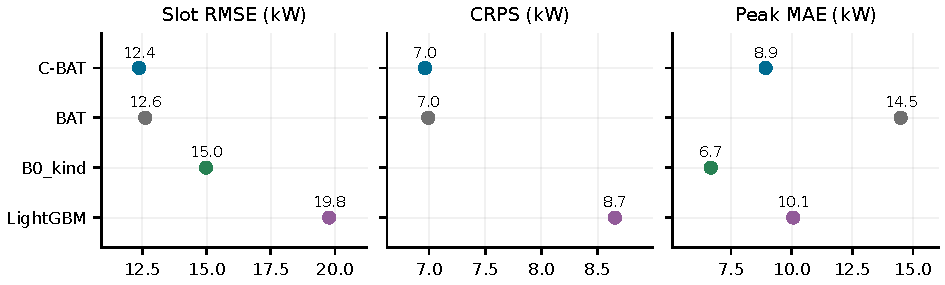
\includegraphics[width=\linewidth]{model_compare.pdf}
\caption{개발 구간 f1--f4의 슬롯 RMSE, CRPS, 일 피크 MAE(kW). 점 위의 숫자는 표~\ref{tab:ch2-dev}의 값이며 LightGBM은 LightGBM(튜닝)이다. B0\_kind는 분포를 내지 않아 CRPS가 없다.}\label{fig:ch2-compare}
\end{figure}

C-BAT의 가장 큰 개선은 일 피크에서 나왔다. 기존 BAT의 피크 MAE 14.50 kW를 8.93 kW로 줄였고 피크 $R^2$는 0.952에서 0.976으로 올랐다. 전체 피크 MAE만 보면 B0\_kind(6.67 kW)가 가장 낮지만, 관측 피크가 학습 기간 $C_{90}$을 넘은 고피크일 13일의 피크 MAE는 C-BAT 4.37 kW, B0\_kind 7.54 kW, 기존 BAT 12.47 kW, LightGBM(튜닝) 18.27 kW로 C-BAT가 가장 낮았다. B0\_kind는 최근의 같은 유형 날을 복사하므로 평범한 날에는 잘 맞지만 과거보다 높게 오르는 날은 따라가지 못한다. 기존 BAT는 비가동일 14일의 피크를 평균 24.59 kW 높게 보았고, 같은 날들에서 C-BAT의 편향은 2.54 kW였다. 대신 C-BAT는 가동일 37일의 피크를 평균 9.74 kW 높게 예측한다(편향은 예측 평균 $-$ 관측). 이 과대예측의 원인은 3.2절에서 분석한다. 피크 시각 적중률은 기존 BAT 0.255, C-BAT 0.203으로 모든 모델이 낮다. 구간은 넓은 쪽으로 치우쳤다. C-BAT 슬롯 90\% 구간의 적중률은 0.990(평균 폭 58.97 kW), 50\% 구간은 0.781(24.58 kW)로 명목값보다 높고, 일 피크 90\% 구간 적중률은 0.948로 명목값에 더 가깝다.

그림~\ref{fig:ch2-examples}은 비가동일, 고피크가 아닌 가동일, 고피크일에서 일 슬롯 MAE가 각 층의 중앙값에 가장 가까운 대표일의 예측이다. 비가동일(8월 5일)에는 C-BAT 중앙값이 관측과 거의 겹쳤고(일 슬롯 MAE 1.76 kW) LightGBM(튜닝)은 08--20시에 관측보다 뚜렷이 높았다. 가동일(7월 16일)에는 C-BAT가 12시와 17시 무렵의 부하 하락을 포함한 하루 모양을 따랐고, 08--12시의 관측은 중앙값보다 높았으나 90\% 구간 안에 있었다. 고피크일(7월 21일)에는 세 모델의 중앙값 곡선이 모두 08--10시와 13--15시의 관측 피크보다 낮았다. 관측 피크는 C-BAT 90\% 구간의 위쪽에 들어왔다. 중앙값 곡선의 최댓값이 아니라 경로 최댓값의 분포로 일 피크를 예측하는 이유가 여기에 있다.

\begin{figure}[htbp]
\centering
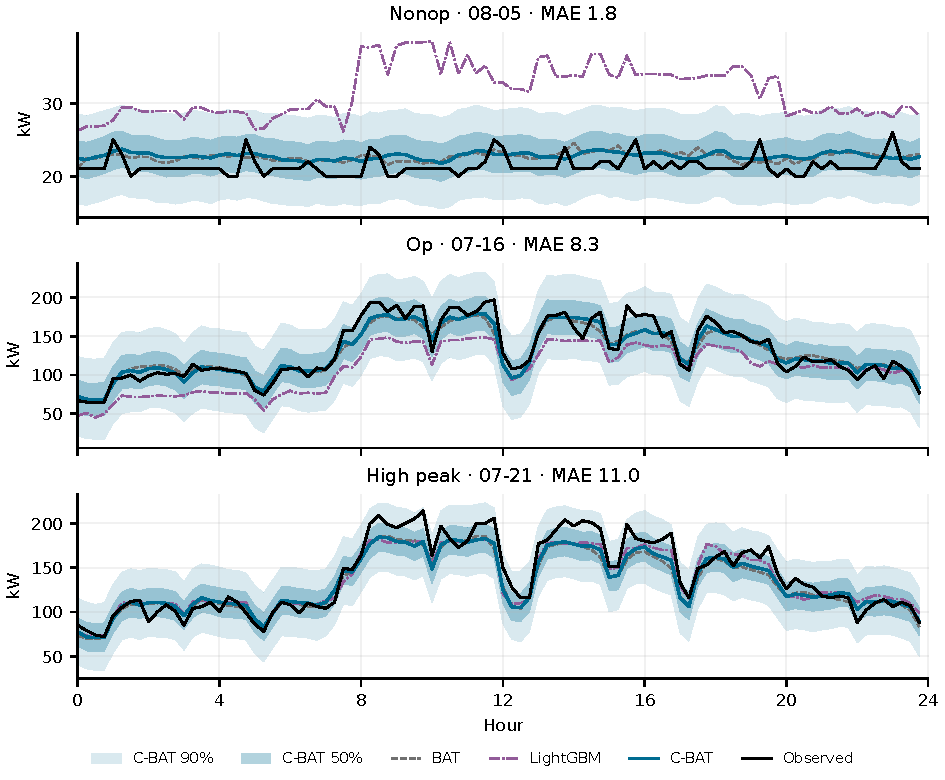
\includegraphics[width=0.86\linewidth]{forecast_examples.pdf}
\caption{층별 대표일의 C-BAT 예측(시드 0). 위부터 비가동일(Nonop, 8월 5일), 고피크가 아닌 가동일(Op, 7월 16일), 고피크일(High peak, 7월 21일)이며 제목의 MAE는 그날 C-BAT의 슬롯 MAE(kW)이다. 검은 선은 관측(Observed), 파란 실선은 C-BAT 중앙값, 짙은·옅은 띠는 C-BAT 50\%·90\% 구간, 회색 파선은 기존 BAT(BAT), 보라색 일점쇄선은 LightGBM(튜닝)의 중앙값이다. 가로축은 시각(Hour)이다.}\label{fig:ch2-examples}
\end{figure}

9월 시험 구간 단독에서는 M2가 C-BAT보다 좋았다(표~\ref{tab:ch2-sept}). M2의 슬롯 MAE는 6.60 kW, CRPS 5.03 kW, 피크 MAE 5.53 kW로 C-BAT(7.18 kW, 5.71 kW, 8.93 kW)보다 낮았다. 슬롯 MAE 차이(C-BAT $-$ M2)는 $+0.58$ kW이고 날짜 단위 부트스트랩 95\% 구간 $[-0.24,\ 1.43]$이 0을 포함해 14일로는 유의하지 않다. 9월에는 고피크일이 하루도 없고 비가동일도 2일뿐이어서 C-BAT의 강점인 고피크일 성능을 시험할 기회가 없었다. C-BAT의 90\% 구간 적중률은 0.984로 개발 구간처럼 구간이 넓었다. 9월은 이전 개발 단계에서 한 번 열린 적이 있어 완전히 독립된 시험이 아니다.

\begin{table}[htbp]
\centering
\hwptablefont
\caption{9월 시험 구간 단독 성능(2021년 9월 1--14일, 1,342슬롯, 피크 평가일 14일, kW).}\label{tab:ch2-sept}
\begin{tabular}{lrrrrrrr}
\toprule
모델 & 슬롯 MAE & RMSE & $R^2$ & CRPS & 90\% 구간 적중 & 피크 MAE & 시각 적중 \\
\midrule
B0 & 7.88 & 11.18 & 0.962 & -- & -- & 7.00 & 0.143 \\
M2 & \textbf{6.60} & 9.75 & 0.971 & \textbf{5.03} & 0.872 & \textbf{5.53} & 0.286 \\
기존 BAT & 6.82 & \textbf{9.53} & \textbf{0.972} & 5.51 & 0.948 & 7.98 & 0.286 \\
C-BAT & 7.18 & 9.79 & 0.971 & 5.71 & 0.984 & 8.93 & 0.286 \\
\bottomrule
\end{tabular}
\end{table}

절제 비교는 C-BAT의 설계 선택을 개발 구간에서 확인한다(표~\ref{tab:ch2-ablation}). 공통 잡음 비교는 학습형 커널 모델에서만 실행했으므로 학습형 커널 행과 비교한다. 잡음을 상태별에서 공통으로 바꾸면 피크 MAE가 9.16 kW에서 15.29 kW로, 고피크일 피크 MAE가 4.38 kW에서 7.80 kW로 커졌다. 다만 두 비교 모형의 최대 split-$\hat R$이 1.308과 2.303으로 기준을 넘으므로 이 차이를 잡음 설계만의 확정된 효과 크기로 보지 않는다. 커널을 학습형으로 바꾸면 슬롯 MAE는 0.17 kW 좋아지고(날짜 단위 구간 $[0.07,\ 0.28]$) 피크 MAE는 0.23 kW 나빠지며 수렴 기준도 넘었다. 이에 따라 수렴이 안정적이고 피크가 조금 나은 고정 커널을 택하였다. 가동유형 기준 기준일(종류 기준)은 슬롯 MAE를 7.80 kW로 낮추지만 피크 MAE(9.06 kW)와 고피크일 피크 MAE(5.02 kW)가 커져 채택하지 않았다. 기존 BAT에서 생산 전달항을 빼도 슬롯 MAE 7.73 kW, 피크 MAE 14.53 kW로 기존 BAT와 거의 같았다. 이 밖에 사전 등록한 확장 실험 11가지는 모두 채택 조건을 넘지 못하였으며 3.4절에 정리하였다.

\begin{table}[htbp]
\centering
\hwptablefont
\caption{절제 비교(개발 구간 f1--f4, 시드 0--2 평균, kW). C-BAT는 상태별 잡음과 고정 커널을 쓴다. 공통 잡음 행은 학습형 커널 행과 비교한다. 기존 BAT 두 행은 split-$\hat R$ 기록이 없다.}\label{tab:ch2-ablation}
\begin{tabular}{lrrrrrr}
\toprule
모델 & 슬롯 MAE & RMSE & CRPS & 피크 MAE & 고피크일 피크 MAE & 최대 $\hat R$ \\
\midrule
C-BAT & 8.50 & 12.37 & 6.96 & \textbf{8.93} & \textbf{4.37} & 1.029 \\
학습형 커널 & 8.34 & \textbf{12.10} & \textbf{6.85} & 9.16 & 4.38 & 1.308 \\
공통 잡음(학습형 커널) & 8.26 & 12.15 & 7.43 & 15.29 & 7.80 & 2.303 \\
종류 기준 기준일 & 7.80 & 12.80 & 6.86 & 9.06 & 5.02 & 1.038 \\
기존 BAT & 7.82 & 12.61 & 6.99 & 14.50 & 12.47 & -- \\
기존 BAT(전달항 없음) & \textbf{7.73} & 12.89 & 7.03 & 14.53 & 12.27 & -- \\
\bottomrule
\end{tabular}
\end{table}

최종모델은 개발 구간 결과로 C-BAT를 선정하였고, 동결한 C-BAT의 성능을 9월까지 합친 합산 평가로 보고한다. 선정 근거는 다음과 같다.
\begin{hwplist}
\item 일 피크: 합산 피크 MAE가 8.93 kW로 네 모델 중 가장 낮고, 기존 BAT·M2 대비 차이의 구간이 0을 포함하지 않는다.
\item 고피크일: 요금과 설비 운용에 가장 중요한 고피크일 13일의 피크 MAE가 4.37 kW로 개발 구간 여섯 모델 중 가장 낮고, 기존 BAT·LightGBM(튜닝) 대비 개선은 두 방식의 구간 모두에서 0을 포함하지 않는다.
\item 확률 예측: 개발 구간 슬롯 RMSE(12.37 kW)와 CRPS(6.96 kW)가 가장 낮다. 일 피크 분포와 초과확률을 같은 경로에서 내며, 점예측만 내는 B0\_kind는 이 산출물(4장 월 최대 갱신 경보의 입력)을 줄 수 없다.
\item 안정성과 단순성: 모든 적합 단계에서 split-$\hat R$이 1.05 이하로 수렴 기준을 만족하였다. 입력은 생산계획, 가동 여부·날짜유형, 과거 전력뿐이며 기상과 공휴일 정보는 쓰지 않는다.
\end{hwplist}
다음 약점과 한계도 함께 밝힌다.
\begin{hwplist}
\item 합산 슬롯 MAE는 기존 BAT(7.61 kW)가 C-BAT(8.22 kW)보다 낮다. 슬롯 곡선만 보면 C-BAT가 최선이 아니다.
\item 개발 구간 전체 피크 MAE는 B0\_kind(6.67 kW)가 C-BAT(8.93 kW)보다 낮고, C-BAT는 가동일 37일의 피크를 평균 9.74 kW 높게 예측한다.
\item 9월 단독에서는 M2가 슬롯 MAE, CRPS, 피크 MAE에서 C-BAT보다 좋았다.
\item 9월 시험 구간은 이전 개발 단계에서 한 번 열린 적이 있어 완전한 미사용 구간이 아니며, 9월에는 고피크일이 0일이어서 고피크일 성능은 개발 구간 13일에서만 확인되었다.
\item 합산 비교는 9월 일별 예측이 있는 네 모델(C-BAT, 기존 BAT, M2, B0)에 한정되며, B0\_kind와 LightGBM(튜닝)에 대한 우위로 확대하지 않는다.
\item 월 최대 갱신 경보의 백테스트에서 갱신일은 1건(7월 19일)뿐이고, 그 133,120원은 완벽한 조치를 가정한 상한이다(4장).
\item 생산계획을 옮겨 얻는다는 모형 반사실 절감액은 관측 유사일 검증에서 지지되지 않아 주장하지 않는다(4장).
\end{hwplist}
따라서 합산 평가의 피크 개선은 성과로 보고하되, 모든 모델과 계절에 대한 우위나 실제 조치 효과로 확대하지 않는다.

\hwpchapter{3}{영향요인 및 오류분석}{15}

개발 구간(f1--f4, 53일, 5,016슬롯, 피크 평가일 51일)에서 C-BAT가 잘 맞는 조건과 틀리는 조건을 구분하였다. 슬롯 오차는 예측 중앙값으로, 일 피크 오차는 사후 경로마다 구한 하루 최댓값(이하 경로 최댓값)의 중앙값으로 계산하였으며, C-BAT 수치는 seed 0--2의 평균이다. 고피크일은 일 피크가 해당 학습 기간 C90을 넘은 13일이다. 지표의 정의는 2.2절을 따른다. 9월 시험 구간은 고피크일이 없고 비가동일이 2일뿐이어서 조건별 분석에는 쓰지 않고 보조로만 언급하였다.

\hwpsection{3.1 생산조건별 예측오차}

슬롯을 그날의 가동유형과 그 슬롯 시각의 계획 생산 여부로 일곱 조건으로 나누어 슬롯 MAE를 비교하였다(표~\ref{tab:ch3-regime}). 비생산은 해당 시각의 계획 생산량이 0인 상태이며 설비 전체의 정지를 뜻하지 않는다. C-BAT 수치는 C-BAT의 조건별 오차 산출 파일에서, 기존 BAT·M2·B0 수치는 같은 개발 구간 예측의 조건별 오차 파일에서 가져왔다. 두 파일의 조건별 관측 슬롯 수는 일곱 조건 모두 같았다(합계 5,016).

\begin{table}[htbp]
\centering
\hwptablefont
\setlength{\tabcolsep}{4pt}
\caption{생산조건별 슬롯 MAE(개발 구간 53일, kW). C-BAT 편향은 예측 중앙값에서 관측을 뺀 값의 평균이다.}\label{tab:ch3-regime}
\begin{tabular}{L{5.4cm}rrrrrrr}
\toprule
 & & & \multicolumn{2}{c}{C-BAT} & & & \\
\cmidrule(lr){4-5}
생산조건 & 관측 슬롯 & 일수 & MAE & 편향 & 기존 BAT & M2 & B0 \\
\midrule
가동유형 0 (비가동) & 1,394 & 15 & 1.73 & $+0.73$ & 1.67 & 4.41 & 34.32 \\
가동유형 1 (1--12시간)·비생산 & 378 & 6 & 7.95 & $-6.14$ & 4.06 & 3.33 & 3.75 \\
가동유형 1 (1--12시간)·생산 & 172 & 6 & 8.69 & $-5.84$ & 7.71 & 11.26 & 17.26 \\
가동유형 2 (13--19시간)·비생산 & 268 & 8 & 20.66 & $+13.67$ & 9.29 & 15.42 & 6.18 \\
가동유형 2 (13--19시간)·생산 & 500 & 8 & 14.52 & $-2.38$ & 16.15 & 17.97 & 28.25 \\
가동유형 3 (20시간 이상)·비생산 & 108 & 16 & 7.98 & $-5.09$ & 8.00 & 18.66 & 29.19 \\
가동유형 3 (20시간 이상)·생산 & 2,196 & 24 & 10.05 & $-2.92$ & 10.30 & 15.43 & 28.90 \\
\midrule
전체 & 5,016 & 53 & 8.50 & -- & 7.82 & 11.64 & 26.84 \\
\bottomrule
\end{tabular}
\end{table}
\hwpnote{관측 슬롯은 목표가 관측된 15분 슬롯 수이고, 일수는 그 조건의 슬롯을 하나 이상 가진 날 수이다. 가동유형 3·비생산은 20시간 이상 가동일 안의 생산 공백 시각으로, 16일에 걸쳐 108슬롯뿐이다. C-BAT는 seed 0--2 평균이고 기존 BAT·M2·B0는 저장된 예측 한 벌이다. 편향이 양수이면 과대예측이다.}

C-BAT의 오차는 비가동일에서 1.73 kW로 가장 작고, 가동유형 2의 비생산 슬롯에서 20.66 kW로 가장 컸다. 이 슬롯의 편향은 $+13.67$ kW로, 13--19시간 가동일의 생산 시작 전과 종료 뒤 전력을 가동 수준으로 높게 예측하였다. 이 조건에서 C-BAT는 네 모형 가운데 가장 나빴고 B0(6.18 kW)보다도 오차가 컸다. C-BAT의 기준일은 가동 여부와 날짜유형만 맞추므로(2.1절) 13--19시간 가동일이 생산 시각이 다른 날의 곡선을 빌려 올 수 있으며, 이를 과대예측의 원인 후보로 보았다. 가동유형 1에서도 C-BAT(7.95, 8.69 kW)는 기존 BAT(4.06, 7.71 kW)보다 오차가 컸고, 편향이 $-6.14$, $-5.84$ kW로 하루 전체를 낮게 예측하였다. 반면 20시간 이상 가동일에서는 생산·비생산 슬롯 모두 C-BAT가 기존 BAT와 같거나 조금 작았고 M2(15.43, 18.66 kW)와 B0보다 작았다. 전체 슬롯 MAE에서 C-BAT(8.50 kW)가 기존 BAT(7.82 kW)보다 큰 것은 대부분 가동유형 2·비생산과 가동유형 1·비생산 슬롯에서 생긴 차이이며, 가동유형 2·생산과 3·생산에서는 C-BAT가 더 작았다.

생산 시작 시각별로는 07시에 시작한 2일의 슬롯 MAE가 21.56 kW(편향 $+17.80$ kW), 08시에 시작한 5일이 13.51 kW로, 전날부터 이어 가동한 20일(10.38 kW)이나 01시에 시작한 11일(9.43 kW)보다 컸다. 07--08시에 시작한 날은 모두 가동유형 2이므로 앞의 비생산 슬롯 과대예측과 같은 현상이다. 하루 중에서는 18시(11.11 kW)와 19시(10.11 kW)의 오차가 가장 크고 21--23시(5.93--6.05 kW)가 가장 작았으며, 08--16시에는 편향이 $-1.42$ kW에서 $-3.83$ kW 사이로 생산 시간의 전력을 조금 낮게 예측하였다. 요일별로는 월요일 8일이 14.10 kW(편향 $+5.22$ kW)로 가장 컸다. 일 생산량 사분위별 슬롯 MAE는 10.07--11.69 kW로 차이가 작아, 슬롯 오차는 생산량의 크기보다 생산 시각의 배치에 따라 갈렸다.

\hwpsection{3.2 일 피크 층별 오차와 개별 날짜}

피크 평가일 51일을 비가동 14일과 가동 37일로 나누고, 가동일에 포함되는 고피크일 13일을 따로 묶어 일 피크 MAE와 편향을 비교하였다(표~\ref{tab:ch3-strata}, 그림~\ref{fig:ch3-strata}). C-BAT의 피크 MAE는 비가동일 2.50 kW, 가동일 11.36 kW, 고피크일 4.37 kW로, 고피크일 오차가 가동일 전체보다 작았다. 기존 BAT는 비가동일 피크를 평균 24.59 kW 높게, LightGBM(튜닝)은 고피크일 피크를 20.37 kW 낮게 예측하였다. C-BAT는 이 두 실패를 함께 줄였으나 가동일 피크를 평균 9.74 kW 높게 예측하였다. B0\_kind는 전체(6.67 kW)·비가동(0.93 kW)·가동(8.84 kW) 피크 MAE가 가장 작았고 고피크일에서는 7.54 kW(편향 $-4.77$ kW)로 C-BAT보다 컸다. 다만 고피크일에서 C-BAT와 B0\_kind의 차이($-3.17$ kW)의 날짜 단위 짝지은 bootstrap 95\% 신뢰구간 [$-7.04$, 0.40]은 0을 포함한다.

\begin{table}[htbp]
\centering
\hwptablefont
\setlength{\tabcolsep}{4pt}
\caption{일 피크 층별 MAE와 편향(개발 구간 피크 평가일 51일, kW). 편향은 경로 최댓값의 평균에서 관측 피크를 뺀 값이다. 고피크일 13일은 가동일 37일에 포함된다.}\label{tab:ch3-strata}
\begin{tabular}{lrrrrrrrr}
\toprule
 & \multicolumn{4}{c}{피크 MAE} & \multicolumn{4}{c}{피크 편향} \\
\cmidrule(lr){2-5}\cmidrule(lr){6-9}
모형 & 전체 & 비가동 & 가동 & 고피크 & 전체 & 비가동 & 가동 & 고피크 \\
\midrule
C-BAT & 8.93 & 2.50 & 11.36 & 4.37 & $+7.77$ & $+2.54$ & $+9.74$ & $-1.08$ \\
기존 BAT & 14.50 & 24.11 & 10.86 & 12.47 & $+8.10$ & $+24.59$ & $+1.87$ & $-12.24$ \\
B0\_kind & 6.67 & 0.93 & 8.84 & 7.54 & $+0.24$ & $+0.36$ & $+0.19$ & $-4.77$ \\
LightGBM(튜닝) & 10.06 & 2.51 & 12.92 & 18.27 & $+1.98$ & $+19.47$ & $-4.64$ & $-20.37$ \\
\bottomrule
\end{tabular}
\end{table}

\begin{figure}[htbp]
\centering
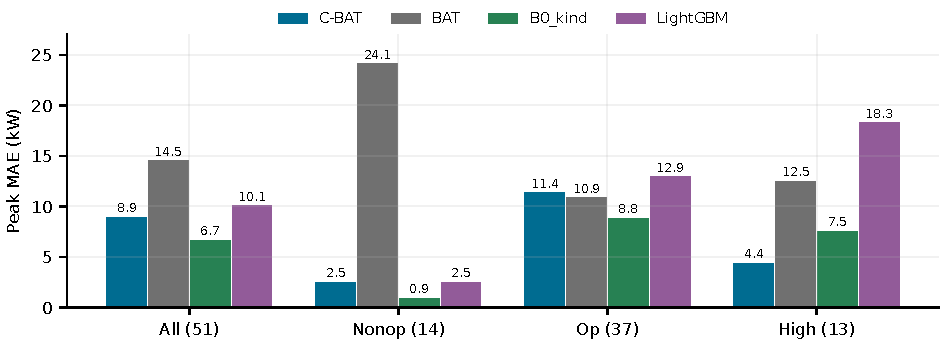
\includegraphics[width=\linewidth]{peak_strata.pdf}
\caption{일 피크 층별 피크 MAE(개발 구간). 가로축은 왼쪽부터 전체 51일(All), 비가동 14일(Nonop), 가동 37일(Op), 고피크 13일(High)이다. 범례의 BAT는 기존 BAT, LightGBM은 LightGBM(튜닝)이며 막대 위 숫자는 MAE(kW)이다.}\label{fig:ch3-strata}
\end{figure}

가동일 과대예측은 평균 곡선이 아니라 경로 최댓값에서 생겼다. 가동일 37일에서 C-BAT 예측 평균 곡선의 하루 최댓값은 관측 피크보다 평균 10.90 kW 낮았다. 경로 최댓값의 중앙값은 여기에 약 20 kW를 더해 가동일 편향(중앙값 기준)을 $+9.22$ kW로 만들었다. 이 추가분은 고피크일에는 알맞았다. 고피크일 13일의 평균 곡선 최댓값은 관측보다 23.51 kW 낮았고, 경로 최댓값을 쓰면 편향이 $-1.70$ kW로 줄었다. 그러나 고피크가 아닌 가동일 24일은 평균 곡선 최댓값의 편향이 $-4.07$ kW뿐이어서, 비슷한 폭을 더한 경로 최댓값의 편향은 $+15.14$ kW가 되었다. C-BAT는 어느 가동일에 피크가 크게 오를지 구분하지 못한 채 모든 가동일에 비슷한 상승폭을 더한 것이다. 슬롯 단위 편향이 음수인 가동유형 1과 3에서도 일 피크 편향(중앙값 기준)이 각각 $+9.86$, $+8.74$ kW로 양수인 것은 이 때문이다. C-BAT는 51일 중 41일, 가동일 37일 중 28일의 피크를 높게 예측하였고, 고피크일 13일 가운데서는 9일을 낮게 예측하였다.

피크 오차가 가장 큰 10일은 모두 고피크가 아닌 가동일이었고, 모두 16.63--31.90 kW 과대예측이었다(표~\ref{tab:ch3-worst}). 관측 피크는 173--195 kW로 각 fold의 C90(198.0--211.0 kW, 1.2절)보다 낮았지만 C-BAT는 204.19--216.19 kW를 예측하였다. 10일 중 7일은 일 슬롯 MAE가 7.38--11.32 kW로 곡선은 대체로 맞았고 피크만 높았다. 일 슬롯 MAE가 큰 8월 16일(25.90 kW)과 7월 9일(22.61 kW)은 가동유형 2이며, 8월 16일은 07시에 시작한 공휴일이다(C-BAT는 공휴일을 입력으로 쓰지 않는다, 1.1절). 10일 중 9일이 8월이었고 그중 8일이 8월 16일 이후였다. 관측 고피크는 7월에 몰리고(22일 중 11일) 8월에는 적었으므로(29일 중 2일), 7월의 높은 피크를 학습한 모형이 8월의 낮아진 피크 수준을 늦게 따라간 것으로 볼 수 있다. 다만 고피크 판정 기준인 C90이 fold마다 달라 생긴 차이가 섞여 있고 표본이 작아 확정하지 않았다.

\begin{table}[htbp]
\centering
\hwptablefont
\setlength{\tabcolsep}{4pt}
\caption{C-BAT 피크 오차 상위 10일(개발 구간, seed 0--2 평균, kW). 시작 0시는 전날부터 이어 가동한 날이다.}\label{tab:ch3-worst}
\begin{tabular}{lcccrrrrr}
\toprule
날짜 & 요일 & 가동유형 & 생산 시작 & 생산시간 & 관측 피크 & 예측 피크 & 피크 오차 & 일 슬롯 MAE \\
\midrule
8월 17일 & 화 & 3 & 0시 & 23 & 173 & 204.90 & $+31.90$ & 8.06 \\
8월 16일 & 월 & 2 & 07시 & 15 & 190 & 215.58 & $+25.58$ & 25.90 \\
7월 9일 & 금 & 2 & 01시 & 18 & 192 & 216.19 & $+24.19$ & 22.61 \\
8월 31일 & 화 & 3 & 0시 & 24 & 187 & 208.35 & $+21.35$ & 11.32 \\
8월 25일 & 수 & 3 & 01시 & 23 & 189 & 210.24 & $+21.24$ & 7.54 \\
8월 27일 & 금 & 3 & 01시 & 23 & 190 & 210.92 & $+20.92$ & 10.47 \\
8월 19일 & 목 & 3 & 0시 & 24 & 188 & 208.57 & $+20.57$ & 7.38 \\
8월 18일 & 수 & 3 & 0시 & 24 & 188 & 207.37 & $+19.37$ & 10.07 \\
8월 30일 & 월 & 2 & 08시 & 16 & 186 & 204.19 & $+18.19$ & 13.43 \\
8월 10일 & 화 & 3 & 01시 & 21 & 195 & 211.63 & $+16.63$ & 7.61 \\
\bottomrule
\end{tabular}
\end{table}
\hwpnote{예측 피크는 경로 최댓값의 중앙값, 피크 오차는 예측 피크에서 관측 피크를 뺀 값이다. 10일 모두 세 seed에서 과대예측이었다. 생산시간은 생산량이 양수인 시간 수이다.}

피크 시각 적중률(실제 피크 시각의 ±2슬롯, 즉 ±30분 이내)은 51일 전체 0.203, 가동일 0.252, 고피크일 0.385였다. 비가동일은 곡선이 평탄하여 0.071에 그쳤고, 기존 BAT의 전체 적중률은 0.255였다. 고피크일의 피크가 08시와 11시에 몰린다는 관측(1.2절)이 있으나 C-BAT는 고피크일 13일 중 5일만 ±30분 안에 맞혔다. 따라서 C-BAT의 일 피크 예측은 크기 판단에 쓰고, 특정 15분 슬롯의 부하를 제어하는 근거로는 쓰지 않았다.

\hwpsection{3.3 피크 기준 초과 경보의 미탐지·오경보}

피크 기준 초과 경보는 그날 일 피크가 C50·C75·C90을 넘을 확률이 문턱 이상일 때 내는 경보이다(기준값과 초과확률의 정의는 2.1절). 개발 구간에서는 fold마다 내부 보정일 7일로 Platt 보정을 적합하고, 같은 fold 내부에서 F1이 가장 큰 확률 문턱을 정하였다. 실제 초과일에 경보가 없으면 미탐지, 초과하지 않은 날에 경보가 나면 오경보로 셌다. 51일 중 초과일은 C50 31일, C75 21일, C90 13일이다(표~\ref{tab:ch3-alarm}).

\begin{table}[htbp]
\centering
\hwptablefont
\caption{피크 기준 초과 경보 성능(개발 구간 51일, 7일 Platt 보정, 확률 모형은 seed 0--2 평균). 매일 경보는 모든 날에 경보를 낸 기준선이다.}\label{tab:ch3-alarm}
\begin{tabular}{llrrrrr}
\toprule
기준(초과일) & 모형 & 정밀도 & 재현율 & F1 & AUC & Brier \\
\midrule
C50 (31일) & C-BAT & 1.000 & 0.882 & 0.937 & 0.997 & 0.020 \\
 & 기존 BAT & 0.967 & 0.935 & 0.951 & 0.976 & 0.020 \\
 & LightGBM(튜닝) & 0.963 & 0.839 & 0.897 & 0.977 & 0.030 \\
 & 매일 경보 & 0.608 & 1.000 & 0.756 & -- & -- \\
\midrule
C75 (21일) & C-BAT & 0.829 & 0.921 & 0.872 & 0.844 & 0.153 \\
 & 기존 BAT & 0.769 & 0.952 & 0.851 & 0.863 & 0.211 \\
 & LightGBM(튜닝) & 0.900 & 0.429 & 0.581 & 0.798 & 0.236 \\
 & 매일 경보 & 0.412 & 1.000 & 0.583 & -- & -- \\
\midrule
C90 (13일) & C-BAT & 0.520 & 0.667 & 0.584 & 0.788 & 0.201 \\
 & 기존 BAT & 0.417 & 0.769 & 0.541 & 0.800 & 0.233 \\
 & LightGBM(튜닝) & 1.000 & 0.231 & 0.375 & 0.688 & 0.253 \\
 & 매일 경보 & 0.255 & 1.000 & 0.406 & -- & -- \\
\bottomrule
\end{tabular}
\end{table}
\hwpnote{매일 경보는 확률을 내지 않으므로 AUC와 Brier를 비워 두었다. C50·C75·C90은 계약전력이나 설비 한계가 아니라 학습 기간 가동일 일 피크의 상대 분위수이다.}

가장 드문 C90에서 C-BAT의 F1은 0.584, Brier는 0.201로 세 확률 모형 가운데 가장 좋았고, AUC(0.788)는 기존 BAT(0.800)보다 조금 낮았다. 기존 BAT는 재현율이 0.769로 높았으나 정밀도가 0.417로 경보 확인 부담이 컸다. LightGBM(튜닝)은 경보를 낸 날은 모두 맞혔지만 재현율이 0.231로 고피크 13일 중 3일만 잡았고, F1(0.375)이 매일 경보(0.406)보다도 낮았다. C75에서도 C-BAT의 F1이 0.872로 가장 높았고, C50에서는 세 모형 모두 F1이 0.89 이상이었다(C-BAT 0.937, 기존 BAT 0.951).

C-BAT의 C90 미탐지(seed 평균 4.33일)는 모두 7월이고 모두 가동유형 3이었으며, 62\%가 일 생산량 상위 25\%에 속하였다. 51일 전체에서 이 세 조건의 비중이 각각 43\%, 47\%, 25\%인 것과 비교하면 한쪽으로 크게 몰렸다. 7월에 생산량이 많은 종일 가동일의 피크가 학습 기간보다 높게 올라갔고 C-BAT가 그 상승을 다 따라가지 못한 것으로 보인다. 오경보(seed 평균 8일)는 7월과 8월이 절반씩이었고, 가동유형 3이 62\%, 가동유형 2가 38\%였다. 요일로는 금요일이 38\%였고 주말 오경보는 없었다. 오경보는 3.2절의 평범한 가동일 과대예측에서 나온 것이다. 미탐지는 여름철 부하 상승을 늦게 따라가서, 오경보는 평범한 가동일의 피크를 높게 보아서 생겼다.

경보 지표는 보정 방식에 민감하였다. 7일 Platt 보정은 적합에 쓸 날이 적다. 개발 구간 C-BAT의 C90 AUC는 보정 전 경로 확률에서 0.926이었으나 보정 뒤 0.788로 떨어졌고, Brier도 0.131에서 0.201로 나빠졌다. C75도 보정 전 Brier(0.146)가 보정 뒤(0.153)보다 낮았으며, C50만 보정 뒤가 조금 나았다(AUC 0.981에서 0.997, Brier 0.021에서 0.020). 최종 실행에서는 8월 말 내부 보정일 7일(쓸 수 있는 날 5일)에 C90 초과일이 없어 보정식이 절편만 추정하였고, 9월 가동일의 C90 위험이 모두 0.0013으로 고정되어 경보가 울릴 수 없었다. 이에 9월 위험 결과를 보기 전에 규칙을 정하여, 최종 발행 확률을 보정 전 경로 확률 $P(\text{경로 최댓값} > C)$로 바꾸었다. 표~\ref{tab:ch3-alarm}은 이전 보정 방식으로 계산한 개발 구간 결과이므로 모형 간 상대 비교로만 읽는다. 보정 전 확률은 평범한 가동일 과대예측을 그대로 이어받아, C90 초과일이 없던 9월에도 C90 위험이 최대 0.30까지 나왔다.

\hwpsection{3.4 위험조건과 보완 대상}

모형과 무관한 관측으로 고피크일의 조건을 보면, 13일은 모두 13시간 이상 가동한 날이었다(1.2절). 가동유형 2는 8일 중 3일(37.50\%), 가동유형 3은 24일 중 10일(41.67\%)이 고피크였고, 가동유형 1의 5일(평균 피크 107.60 kW)과 비가동일에는 고피크가 없었다. 피크 평가일 가운데 전날부터 이어 가동한 19일은 고피크 비율이 42.11\%이고 피크가 가장 자주 나온 시각이 11시였으며, 07--08시에 시작한 7일은 3일이 고피크이고 피크가 주로 08시에 나왔다. 01시에 시작한 11일은 고피크 비율이 18.18\%로 낮았다. 금요일은 7일 중 1일(14.29\%)만 고피크였고 토·일요일에는 고피크가 없었다. 일 생산량 1사분위(평균 피크 153.60 kW)를 빼면 2--4사분위의 평균 피크는 198.56--202.67 kW로 비슷하여, 생산량이 많을수록 피크가 계속 커지지는 않았다.

같은 조건 안에서 고피크일과 평범한 가동일을 가르는 신호는 약하였다. 가동일 37일에서 C-BAT 피크 오차(경로 최댓값의 중앙값에서 관측을 뺀 값, seed 평균)와 생산 시작 시각의 선형 상관은 $r=-0.03$, 생산 첫 2시간의 생산량 비중과는 $r=-0.01$, 생산시간과는 $r=-0.01$이었다. 이 세 특성의 선형 관계로는 오차가 큰 날을 구분할 수 없었다. 특성의 조합이나 비선형 관계는 따로 검증하지 않았으므로, 이 결과만으로 생산계획에 고피크 정보가 없다고 판단하지는 않았다.

생산계획 입력 오차의 영향은 학습 입력과 채점할 실제 전력을 그대로 두고 예측일에 넣는 계획만 바꾸어 확인하였다. 생산량 오차는 평균이 1인 로그정규 배수(로그 표준편차 0.05, 0.1, 0.2, 날짜별 10회 반복)로, 시각 오차는 계획 전체를 1시간 앞당기거나 늦추어 넣었다. C-BAT는 seed 0 하나로 실행하였다(표집 6,000회, burn-in 3,000회). 오차가 없을 때 8.49 kW였던 C-BAT 슬롯 MAE는 로그 표준편차 0.2에서도 8.50 kW로 0.04\% 늘었다. 계획을 1시간 이르게 넣으면 8.78 kW($+3.35$\%), 늦게 넣으면 8.64 kW($+1.77$\%)가 되었다. 기존 BAT($+0.44$, $+0.06$ kW)와 LightGBM(튜닝)($+0.87$, $+0.69$ kW)도 생산량 오차보다 시각 오차에 더 민감하였다. C-BAT의 피크 MAE는 모든 조건에서 8.61--8.94 kW였다. 전력이 생산량의 크기보다 가동 여부와 가동 시각을 따른다는 3.1절의 결과와 맞으며, 현장에서는 생산량보다 가동 시작·종료 시각의 입력 정확도가 중요하다. 계획 취소나 설비 고장처럼 가동 여부 자체가 바뀌는 경우는 시험하지 않았다.
\hwpnote{기존 BAT와 LightGBM(튜닝)의 입력 오차 결과는 같은 코드와 절차로 앞서 실행한 결과(표집 2,000회)를 옮겼다. 괄호 안 값은 오차가 없을 때 대비 슬롯 MAE 증가분이며, 앞이 1시간 이르게, 뒤가 1시간 늦게 넣은 경우이다.}

C-BAT의 구성을 바꾸어 보는 확장 실험 11가지를 사전 등록하여 개발 구간에서만 평가하였고, 채택된 것은 없다(표~\ref{tab:ch3-ext}). 각 실험은 결과를 보기 전에 채택 조건을 문서로 고정하였다. 조건은 실험마다 조금씩 다르지만 공통으로 C-BAT의 전체 피크 MAE(8.93 kW)와 고피크일 피크 MAE(4.37 kW)를 지키면서 곡선이나 가동일 편향을 개선하도록 요구하였다. 9월 시험 구간은 쓰지 않았다.

\begin{table}[htbp]
\centering
\hwptablefont
\setlength{\tabcolsep}{4pt}
\caption{사전 등록 확장 실험(개발 구간 f1--f4, seed 0--2 평균, kW). 앙상블은 C-BAT seed 0과 비교하였고 fold 하나씩 뺀 가중치로 평가하였으며, 일 피크는 C-BAT와 같다.}\label{tab:ch3-ext}
\begin{tabular}{L{1.4cm}L{4.1cm}rrrL{4.1cm}}
\toprule
분류 & 변형 & 슬롯 MAE & 피크 MAE & 고피크 MAE & 미충족 조건 \\
\midrule
기준 & C-BAT & 8.50 & 8.93 & 4.37 & -- \\
\midrule
잡음 & 가동유형별 4상태 잡음 & 8.76 & 9.18 & 6.50 & 가동일 편향, 고피크 \\
 & 슬롯 4상태 잡음 & 8.96 & 10.47 & 6.80 & 가동일 편향, 예측 구간 적중률, 고피크 \\
 & Student-$t$ 혁신 & 8.70 & 9.90 & 4.53 & 가동일 편향, 예측 구간 적중률 \\
 & 가동유형별 잡음 + $t$ 혁신 & 8.99 & 10.49 & 7.30 & 네 조건 모두 \\
\midrule
기준일 & 가동유형 기준 & 7.80 & 9.06 & 5.02 & 전체 피크 \\
 & 시간별 계획 기준 & 7.63 & 9.80 & 5.16 & 가동일 편향, 고피크 \\
 & 어텐션 기준일, 전달항 없음 & 7.92 & 11.69 & 4.85 & 전체 피크 \\
 & 어텐션 기준일 + 전달항 & 7.76 & 11.93 & 4.57 & 전체 피크 \\
\midrule
피크 계층 & v1 기준일 피크 회귀 & 7.76 & 11.85 & 21.70 & 전체 피크, 고피크 \\
 & v2 C-BAT 피크 사전 & 7.76 & 12.27 & 20.73 & 전체 피크, 고피크 \\
\midrule
앙상블 & M2 + C-BAT & 8.82 & -- & -- & 슬롯 MAE(C-BAT 8.49) \\
\bottomrule
\end{tabular}
\end{table}
\hwpnote{예측 구간 적중률 조건은 슬롯 90\% 예측 구간 적중률이 0.90에 더 가까워질 것을 요구하였다. 어텐션 기준일은 과거 28일 완전 관측일의 곡선을 시간별 가동 여부와 날짜유형의 유사도로 가중평균한 기준곡선이고, 피크 계층은 C-BAT 곡선과 별도로 일 피크를 회귀로 예측한 2계층 구조이다. 이 실험들은 개발 구간을 다시 쓴 탐색적 결과이다.}

확장 실험은 곡선이나 한 층만 개선하였고 C-BAT의 피크 균형을 넘은 변형은 없었다. 기준일을 바꾼 네 실험은 슬롯 MAE를 7.63--7.92 kW로 낮추었지만 피크 MAE가 9.06--11.93 kW로 커졌다. 어텐션 기준일 두 모형은 가동일 편향(평균 기준)을 C-BAT의 $+9.74$ kW에서 $+14.26$, $+14.74$ kW로 키웠다. 잡음 변형 4종은 예측 구간을 넓혀 경로 최댓값을 더 끌어올렸고, 가동일 편향(중앙값 기준)이 $+9.22$ kW에서 $+9.38$--$+12.45$ kW로 오히려 커졌다. 전용 피크 계층은 비가동일 피크 MAE(v1 1.07 kW)와 C90 경보 F1(v1 0.686)을 개선하였으나, 회귀가 가동일 피크를 평균 쪽으로 수축시켜 고피크일을 20 kW 넘게 낮게 보았다. M2와의 점예측 앙상블은 fold마다 고른 M2 가중치가 0.05--0.30으로 흔들렸고, fold 하나씩 뺀 슬롯 MAE가 8.82 kW로 C-BAT(8.49 kW)보다 나빴다. 시험한 입력과 모형에서는 평범한 가동일의 과대예측을 줄이면서 고피크일 성능을 유지하는 방법을 찾지 못하였다.

이상의 오류분석에서 다음 보완 대상을 정하였다.
\begin{hwplist}
\item 평범한 가동일의 피크 과대예측: 경로 최댓값이 모든 가동일에 약 20 kW의 상승폭을 비슷하게 더하는 것이 주원인이다. 시험한 생산계획 특성과 모형 변형으로는 고피크일과 평범한 가동일을 구분하지 못하였으므로, 이 자료에 없는 설비별 가동 여부·제품 종류·교대조 정보(1.2절)를 확보하여 다시 검증해야 한다.
\item 13--19시간 가동일의 생산 시작 전·종료 뒤 슬롯: C-BAT가 네 모형 중 가장 큰 오차(20.66 kW)를 낸 조건이다. 기준일을 가동유형이나 시간별 계획으로 고르면 곡선은 좋아졌으나 피크가 나빠졌으므로, 곡선 개선과 피크 균형을 함께 만족하는 기준일 규칙이 필요하다.
\item 1--12시간 가동일의 과소예측: 슬롯 편향이 $-5.84$, $-6.14$ kW이고 기존 BAT보다 오차가 컸다. 개발 구간에 6일뿐이므로 표본을 늘려 다시 확인한다.
\item 계절에 따른 피크 수준 변화: 7월의 C90 미탐지와 8월 하순의 과대예측은 모두 피크 수준의 변화를 늦게 따라간 결과로 보인다. 운영 중 최근 관측 피크와 예측 피크의 차이를 감시하고, 학습 자료가 쌓이면 다시 추정한다.
\item 경보 확률의 보정: 7일 Platt 보정이 불안정하여 발행은 보정 전 경로 확률로 하였다. 보정 전 확률은 평범한 가동일에서 높게 나오므로 경보 문턱은 미탐지와 오경보의 비용을 함께 반영하여 정하고, 문턱 결정에 쓰지 않은 기간에서 확인해야 한다.
\item 생산계획 입력: 시각 오차의 영향이 생산량 오차보다 크므로 현장 적용 시 가동 시작·종료 시각을 정확히 입력하고 계획과 실적의 차이를 기록한다.
\end{hwplist}
\hwpnote{조건별 표본이 작고(고피크일 13일, 07--08시 시작 7일, 가동유형 1 6일) 조건별 차이의 신뢰구간은 계산하지 않았다. 개발 구간은 모형 선택에도 쓰였으므로 이 장의 결과는 탐색적이며, 관측된 차이를 인과요인이나 다른 기간의 성능으로 일반화하지 않았다.}

\hwpchapter{4}{현장 활용방안}{10}

\hwpsection{4.1 예측 결과의 현장 활용}

C-BAT는 매일 00:00에 당일의 시간별 생산계획과 전날까지 관측된 전력으로 하루 96슬롯의 예측 경로(사후 표본)를 만들고, 이 경로에서 점검에 필요한 값을 뽑아 일일 보고로 낸다(표~\ref{tab:ch4-report}). 보고는 설비 담당자가 어느 시간대와 어느 날을 먼저 점검할지 정하는 데 쓰며, 경보만으로 설비를 자동 제어하거나 정지시키지 않는다.

\begin{table}[htbp]
\hwptablefont
\setlength{\tabcolsep}{4pt}
\caption{00:00 일일 보고의 항목과 읽는 방법.}\label{tab:ch4-report}
\begin{tabular}{L{2.5cm}L{4.4cm}L{3.8cm}L{4.4cm}}
\toprule
항목 & 내용 & 현장에서 쓰는 방법 & 읽을 때의 한계 \\
\midrule
분위수 곡선 & 슬롯별 예측 분위수 19개(5\%p 간격, 5--95\%) & 부하가 높아질 시간대와 불확실한 시간대를 보고 그 시간의 생산량과 설비 동시 가동을 점검 & 슬롯 90\% 구간 적중률이 개발 구간에서 0.990으로 명목값보다 높아 구간이 넓다 \\
일 피크 분포 & 경로별 하루 최댓값의 분포(중앙값, 평균) & 그날 일 피크의 수준과 불확실성 확인 & 일 피크 90\% 구간 적중률 0.948, 평균 폭 49.18 kW(개발 구간) \\
피크 시각 & 경로별 피크 시각의 최빈값 & 점검할 시간대의 후보 & 관측 피크 시각의 $\pm$30분 안에 든 비율이 0.203(개발 구간)이라 시각을 단정하지 않는다 \\
피크 기준 초과 확률 & 일 피크가 C50·C75·C90을 넘는 경로의 비율(보정하지 않음) & 점검할 날의 우선순위(3장의 피크 기준 초과 경보) & 7월 종일 가동일의 미탐지와 평범한 가동일의 오경보가 남는다(3장) \\
기준선 $B_d$ & 예측일 00:00에 알려진 요금 적용 최대(4.2절) & 월 최대 갱신 여부를 가르는 기준 & 이전 자료만 쓰며, 갱신이 일어나면 다음 날부터 올라간다 \\
$P_d$, $E_d$ & 경로 최댓값이 $B_d$를 넘을 확률 $P_d$와 넘은 만큼의 기본요금 기댓값 $E_d$(4.2절) & 월 최대 갱신 경보 & 갱신일이 1일뿐이어서 사례로만 읽는다 \\
\bottomrule
\end{tabular}
\end{table}

이 값들은 시간별 생산계획을 미리 안다는 가정(1.4절)에서 나왔다. 계획 입력에 오차를 넣은 실험에서 C-BAT의 슬롯 MAE는 생산량 오차(로그 표준편차 0.2)에서 0.04\% 늘었고 계획 전체를 1시간 이르게 넣으면 3.3\% 늘었다. 현장에서는 생산량보다 가동 시작·종료 시각의 계획 정확도가 더 중요하다. 계획 취소나 설비 고장처럼 가동 여부 자체가 바뀌는 경우는 시험하지 않았다.

\hwpsection{4.2 월 최대 갱신 경보 규칙과 백테스트}

기본요금은 매달 요금 시간대의 최대수요와 래칫 바닥 가운데 큰 값(청구 수요)에 1 kW당 8,320원(2021년 산업용(을) 요금표)을 곱해 정해진다. 요금 시간대는 일요일과 공휴일을 뺀 09--23시이고, 래칫 바닥은 지난 1년 동안 래칫 적용월(12·1·2·7·8·9월)의 최대수요에서 온다. 따라서 기본요금을 움직이는 날은 그 달의 최대를 새로 쓰는 날뿐이다. 이 장에서는 이 날을 월 최대 갱신일, 그 위험을 당일 00:00에 알리는 경보를 월 최대 갱신 경보라 한다. 이 경보는 일 피크가 C50·C75·C90을 넘을 확률로 내는 3장의 피크 기준 초과 경보와 기준이 다르다.

경보 규칙은 백테스트 결과를 보기 전에 문서로 정해 두었고, 예측일 $d$의 00:00에 다음 순서로 계산한다.
\begin{hwplist}
\item 기준선: 이번 달 1일부터 전날까지의 요금 시간대 관측 최대와, 이번 달 이전 1년 안 래칫 적용월의 요금 시간대 관측 최대 가운데 큰 값을 기준선 $B_d$로 둔다. $d$일 이전 관측만 쓴다.
\item 경로 최댓값: C-BAT의 사후 경로 $s=1,\dots,S$마다 요금 시간대 슬롯의 최댓값 $M_d^{(s)}$를 구한다.
\item 위험: 갱신 확률 $P_d$와 기대 초과 기본요금 $E_d$를 식~\eqref{eq:ch4-pe}로 구한다. 시드 3개(0·1·2)의 값을 평균한다.
\item 경보: $E_d$가 점검 비용 3만 원(담당자 1--2시간 가정) 이상이면 경보한다(주 규칙). 1만 원, 10만 원, $P_d \ge 0.5$는 민감도로 본다.
\end{hwplist}
\begin{equation}
P_d = \frac{1}{S}\sum_{s=1}^{S} \mathbf{1}\bigl[M_d^{(s)} > B_d\bigr], \qquad
E_d = 8{,}320 \times \frac{1}{S}\sum_{s=1}^{S} \max\bigl(0,\ M_d^{(s)} - B_d\bigr).
\label{eq:ch4-pe}
\end{equation}
위험은 Platt 보정을 거치지 않은 경로 비율을 그대로 쓴다. 보정에 쓰는 최근 7일 안에 C90 초과일이 없으면 보정식이 절편만 추정되어 모든 날의 위험이 같은 값이 되기 때문이다. 개발 구간에서도 C90의 AUC는 보정 전 0.926에서 보정 뒤 0.788로 낮아졌다.

백테스트는 시뮬레이션이 아니라 과거 각 날에 규칙을 적용하고 실제 관측으로 채점한 것이다. 대상은 개발 구간(2021년 7월 7일--8월 31일) 가운데 요금 시간대 관측이 있는 44일이며, 이 중 월 최대 갱신일은 7월 19일 하루였다. 그날 요금 시간대 최대는 222 kW로 전날까지의 기준선 206 kW를 16 kW 넘었고, 기본요금 8,320원/kW를 적용하면 그 달 기준 133,120원이다. 주 규칙은 이날을 잡았고 44일 동안 10번 경보하였다(표~\ref{tab:ch4-alarm}). 기준일 곡선을 그대로 쓰는 B0\_kind는 이날을 놓쳤다.

\begin{table}[htbp]
\centering
\hwptablefont
\caption{월 최대 갱신 경보 백테스트(개발 구간 중 요금 시간대 관측이 있는 44일, 갱신일 1일).}\label{tab:ch4-alarm}
\begin{tabular}{lcrrr}
\toprule
규칙 & 갱신일 포착 & 경보 수 & 오경보 & 금액 상한(원) \\
\midrule
$E_d \ge$ 1만 원 & 1/1 & 23 & 22 & 133,120 \\
$E_d \ge$ 3만 원(주 규칙) & 1/1 & 10 & 9 & 133,120 \\
$E_d \ge$ 10만 원 & 1/1 & 3 & 2 & 133,120 \\
$P_d \ge 0.5$ & 1/1 & 3 & 2 & 133,120 \\
C-BAT 점예측 $> B_d$ & 1/1 & 3 & 2 & 133,120 \\
B0\_kind 기준일 $> B_d$ & 0/1 & 0 & 0 & 0 \\
매일 경보 & 1/1 & 44 & 43 & 133,120 \\
\bottomrule
\end{tabular}
\end{table}
\hwpnote{금액 상한은 갱신일의 초과분을 완벽한 조치로 모두 막았다고 가정한 그 달 기준 값이며 실제 절감액이 아니다. C-BAT 점예측은 경로 최댓값의 중앙값이다. 2020년 12월 자료가 없어 기준선에는 그 달의 최대가 들어 있지 않다.}

7월 19일에 C-BAT는 갱신 확률 $P_d=0.58$, 기대 초과 기본요금 $E_d=122{,}919$원, 경로 최댓값의 중앙값 211.19 kW를 냈다. B0\_kind의 기준일 곡선은 이날 요금 시간대 최대를 195 kW로 두어 기준선에 못 미쳤다. 점검 비용 기준을 10만 원으로 올리면 경보는 3번으로 줄지만 갱신일은 여전히 잡힌다. 오경보 9건 가운데 6건은 7월 7--16일에 몰려 있다. 이 기간 관측 피크는 187--201 kW였으나 C-BAT 경로 최댓값의 중앙값은 201.56--214.65 kW로 기준선 206 kW 부근이었다. 기준선이 평소 가동일 피크와 가까웠고, 평범한 가동일의 피크를 높게 예측하는 C-BAT의 경향(3장)이 겹친 결과이다. 갱신일이 1일뿐이므로 이 결과는 성능 추정이 아니라 사례이다.

\hwpsection{4.3 경보일 점검 항목과 금액 해석}

경보일에는 다음 항목을 점검한다. 항목은 관측 조건에서 정한 것이며 저감 효과는 검증하지 않았다. 최종 적용은 설비·작업 순서·납기를 아는 담당자가 정한다.
\begin{hwplist}
\item 초반 부하: 유사일 비교에서 초반 두 시간의 생산 비중이 10\%p 높은 날은 요금 시간대 피크가 9.3 kW 높았다. 실제 설비 가동 기록으로 동시 기동 여부를 확인하고, 작업 제약이 허용하면 기동 순서를 분산하는 조치를 시험한다.
\item 08시·11시 부하 집중: 개발 구간 고피크일 13일 가운데 10일(08시 6일, 11시 4일)이 두 시각 중 하나에 피크를 기록하였다(1.2절). 이 집계만으로 동시 기동이 원인이라고 단정하지 않는다. 08시는 요금 시간대 밖이라 기본요금 산정에 들어가지 않고, 11시는 여름철 최대부하 시간대로 산정에 들어간다.
\item 기준선 근접 시 비필수 부하 지연: 당일 요금 시간대 부하가 $B_d$에 가까워지면 비필수 부하를 뒤로 미룬다.
\end{hwplist}

초반 부하 항목의 방향은 모형과 무관한 유사일 비교에서 얻었다. 2021년 9월 이전 가동일 89일에서 가동유형과 날짜유형이 같고 일 생산량 차이가 10\% 이내인 날로 쌍을 만들고, 시작 시각이나 초반 생산 비중만 다른 쌍의 실측 요금 시간대 피크를 비교하였다. 시작 시각이 1시간 이상 다른 206개 쌍에서는 늦게 시작한 날의 피크가 평균 11.1 kW 높았다(95\% 구간 $[5.2,\ 17.4]$). 피크 차이의 합을 시작 지연 시간의 합으로 나눈 값은 1시간당 7.4 kW였다(95\% 구간 $[3.4,\ 12.0]$). 그러나 쌍별 피크 차이의 중앙값은 2.0 kW로, 큰 차이는 일부 쌍에 몰려 있다. 시작 시각이 같고 초반 두 시간의 생산 비중이 5\%p 이상 다른 쌍은 25개뿐이었고 10\%p당 9.3 kW였다(95\% 구간 $[0.6,\ 20.2]$). 한 날이 여러 쌍에 들어가 구간은 실제보다 좁을 수 있고, 시작 시각은 수주량이나 설비 상태와 함께 움직일 수 있다. 따라서 이 값은 관측된 연관성이며 조치의 효과 크기로 쓰지 않는다.

금액은 갱신일을 완벽하게 막았다고 가정한 상한과 점검 비용을 나란히 놓고 읽는다. 주 규칙의 경보일 집합을 $\mathcal A$, 월 최대 갱신일 집합을 $\mathcal E$, 갱신일 $d$의 요금 시간대 관측 최대를 $M_d^{\mathrm{obs}}$라 하면 그 달 기준 계산은 다음과 같다.
\begin{align}
U_{\mathrm{month}} &= 8{,}320\sum_{d\in\mathcal A\cap\mathcal E}
\bigl(M_d^{\mathrm{obs}}-B_d\bigr)^+ = 133{,}120\ \text{원},\notag\\
K_{\mathrm{inspect}} &= 30{,}000\times|\mathcal A| = 30{,}000\times 10 = 300{,}000\ \text{원},\label{eq:ch4-cost}\\
U_{\mathrm{month}} - K_{\mathrm{inspect}} &= -166{,}880\ \text{원}.\notag
\end{align}
이는 점검 비용을 10번의 경보일마다 실제로 지출하고, 포착한 갱신일의 초과분을 전부 막는 경우의 계산이다. 당월 계산만으로는 순편익이 양수라는 근거가 없다. 7월은 래칫 적용월이어서 7월 19일의 초과분은 이후 달의 청구 수요에도 영향을 줄 수 있다. 실제로 8월 요금 시간대 최대는 207 kW였지만 8월 청구 수요는 7월이 만든 222 kW였다. 이 이후 달 영향은 이후 달의 실제 피크에 따라 달라지므로 금액에 넣지 않았다. 점검 시간, 조치 비용, 후속 월 청구 수요는 현장에서 기록해 순편익을 평가해야 한다.
\hwpnote{133,120원은 초과분 16 kW 전체를 줄이는 느슨한 상한이다. 7월의 다음 최대는 7월 21일의 214 kW여서 7월 19일만 낮추면 7월 청구 수요는 214 kW까지 내려가며, 이 경우 감소분은 8 kW $\times$ 8,320원 = 66,560원이다.}

\hwpsection{4.4 적용 절차와 효과 확인}

모형이 계산하는 시간대 이동의 반사실 절감액은 현장 금액으로 쓰지 않았다. 시간대 이동은 가동 시작 시각을 앞이나 뒤로 옮기는 등 하루 총생산량은 두고 생산계획만 바꾸는 변경이다. C-BAT에서 생산계획만 바꾸어 곡선을 다시 계산하면 절감액을 낼 수 있으나, 그 금액이 관측과 맞는지 먼저 확인하였다. 4.3절의 유사일 쌍 231개(206개 + 25개)에서 두 날의 실측 차이와, 두 날의 계획을 서로 바꿔 넣은 모형 차이를 같은 요금 달력으로 비교하였다. 전력량(kWh)은 슬롯 전력(kW)에 0.25시간을 곱해 합한 값이고, 전력량요금은 여기에 시간대별 단가를 곱한 요금이다. 결과는 표~\ref{tab:ch4-counter}와 같다.

\begin{table}[htbp]
\centering
\hwptablefont
\setlength{\tabcolsep}{4pt}
\caption{유사일 231쌍에서 모형 차이와 실측 차이의 비교(늦게 시작하거나 초반 생산 비중이 높은 날 $-$ 비교 날).}\label{tab:ch4-counter}
\begin{tabular}{lrrrl}
\toprule
대상 & 실측 평균 & 모형 평균 & 상관 & 기울기 [날짜 단위 95\% 구간] \\
\midrule
전력량요금 (원/일) & $+7{,}359$ & $-464$ & $-0.01$ & $-1.39$ [$-15.35$, 8.25] \\
요금 시간대 피크 (kW) & $+11.0$ & $+0.2$ & 0.18 & 9.51 [$-10.39$, 19.09] \\
\bottomrule
\end{tabular}
\end{table}
\hwpnote{기울기는 실측 차이를 모형 차이에 원점 회귀한 값으로, 모형 값에 몇 배를 곱해야 실측과 맞는지를 나타낸다. 구간은 날짜 단위 cluster 부트스트랩이며 쌍 단위 구간은 각각 $[-5.06,\ 2.13]$, $[0.07,\ 14.40]$이다. C-BAT는 9월 이전 전체 자료로 한 번 적합하였으므로 쌍의 날짜가 학습에 들어 있는 표본 내 검증이다.}

전력량요금은 상관이 0에 가깝고 평균 방향도 반대여서, 실측에서는 늦게 시작하거나 초반 생산 비중이 높은 날이 하루 7,359원 비쌌지만 모형은 464원 싸다고 계산하였다. 요금 시간대 피크는 모형의 평균 반응이 0.2 kW로 실측 차이 11.0 kW에 크게 못 미쳤고, 날짜 단위 구간이 0을 포함하였다. 실측 쌍은 계획 외의 조건도 다를 수 있어 인과 기준값은 아니다. 그래서 모형이 틀렸다고 결론짓지 않고, 모형 절감액을 관측으로 뒷받침할 수 없다는 데서 멈춘다.

실제 기본요금 규칙을 적용해도 같은 결론이다. 모형이 요금 시간대 피크 감소를 이유로 시간대 이동을 제안한 날은 C-BAT에서 7월 0일, 8월 1일이었다. 7월 청구 수요 222 kW를 정한 7월 19일은 이 날들에 들지 않아 7월 기본요금은 변하지 않는다. 8월은 7월이 만든 래칫 222 kW가 청구 수요를 정해 8월 피크를 얼마나 낮추든 기본요금이 같다. 그래서 두 달의 기본요금 변화는 모두 0원이었고, 모형의 피크 감소를 10배로 키워도 0원이었다. 이에 따라 이 보고서의 금액 주장은 관측된 요금 구조, 즉 갱신일 하루가 만든 금액 상한까지로 제한한다.

조치의 효과는 현장 운영으로 검증한다. 작업 제약이 허용하는 경보일을 사전에 정한 무작위 배정으로 조치일과 비조치일에 나누고, 가동유형과 계획 생산량을 함께 기록하여 두 집단의 요금 시간대 피크를 비교한다. 갱신일이 드물어 비교 지표는 갱신 여부보다 경보일의 요금 시간대 피크를 우선한다. 조치하기 쉬운 날만 고르지 않도록 배정 규칙과 미이행 사유를 남기고, 실제 점검 비용과 조치 비용을 포함한 순편익도 기록한다. 도입은 다음 세 단계로 진행한다.
\begin{hwplist}
\item 1단계(매일 00:00): 당일 생산계획으로 C-BAT를 실행해 분위수 곡선, 일 피크 분포, 피크 시각, $B_d$, $P_d$, $E_d$를 담은 일일 보고를 만든다.
\item 2단계(경보일): 담당자가 보고를 확인하고 설비·작업 순서·납기를 고려하여 4.3절의 점검 항목 가운데 적용할 것을 정한다. 무작위 배정 결과와 적용 여부, 내용을 기록한다.
\item 3단계(매월 말): 경보 수, 오경보, 갱신일 포착 여부, 조치일과 비조치일의 요금 시간대 피크를 검토하고 점검 비용 기준을 조정한다.
\end{hwplist}
\hwpnote{이 장의 경보 백테스트는 개발 구간 중 요금 시간대 관측이 있는 44일에 한정하며, 합산 평가(67일)의 피크 예측 성능과 구별한다. 월 최대 갱신 사례는 1건이어서 경보 규칙의 성능을 추정하지 않았다.}

\hwpchapter{5}{창의성 및 차별성}{10}

\hwpsection{5.1 생산운영 특성을 반영한 예측 성능 개선}

C-BAT는 시간별 생산계획에서 생산 여부와 정규화 로그 생산량을 구분해 입력하고, 가동유형별 기본 곡선, 최근 기준일 곡선, 생산 전달항에 가동·비가동 상태별 날짜 효과와 AR(1) 슬롯 잡음을 더해 하루 경로의 분포를 만든다(2.1절). 분위수, 일 피크 분포, 초과 확률이 모두 같은 경로에서 나온다. 잡음을 가동 상태별로 나눈 것은 1.2절에서 본 비가동일과 가동일의 부하 차이를 반영한 설계이다.

개발 구간과 9월 시험 구간을 합친 합산 평가(피크 평가일 65일)에서 일 피크 MAE는 C-BAT 8.93 kW, 기존 BAT 13.09 kW, M2 14.54 kW였다. 기존 BAT보다 31.8\%, M2보다 38.6\% 낮고, 날짜 단위 짝지은 부트스트랩의 95\% 구간이 두 차이 모두 0을 포함하지 않는다(표~\ref{tab:ch5-pooled}). 개발 구간에서는 비가동일의 일 피크 MAE가 C-BAT 2.50 kW, 기존 BAT 24.11 kW였고, 고피크일 13일의 일 피크 MAE는 C-BAT 4.37 kW, 기존 BAT 12.47 kW, LightGBM(튜닝) 18.27 kW였다. 기존 BAT는 비가동일의 피크를 높게, LightGBM(튜닝)은 고피크일의 피크를 낮게 보았고 C-BAT는 두 실패를 모두 줄였다. 고피크일 차이의 95\% 구간은 기존 BAT 대비 $-8.10$ kW $[-11.19,\ -5.80]$, LightGBM(튜닝) 대비 $-13.90$ kW $[-19.01,\ -9.86]$이다.

\begin{table}[htbp]
\centering
\hwptablefont
\setlength{\tabcolsep}{4pt}
\caption{합산 평가의 C-BAT와 비교 모델(피크 평가일 65일, 6,358슬롯, kW). 차이는 C-BAT $-$ 비교 모델이며 대괄호는 날짜 단위 짝지은 부트스트랩 95\% 구간이다.}\label{tab:ch5-pooled}
\begin{tabular}{llrrl}
\toprule
지표 & 비교 모델 & C-BAT & 비교 모델 & 차이 \\
\midrule
일 피크 MAE & 기존 BAT & 8.93 & 13.09 & $-4.17$ [$-6.95$, $-1.31$] \\
 & M2 & 8.93 & 14.54 & $-5.61$ [$-10.24$, $-1.38$] \\
 & B0 & 8.93 & 34.63 & $-25.70$ [$-42.10$, $-11.43$] \\
\midrule
슬롯 MAE & 기존 BAT & 8.22 & 7.61 & $+0.61$ [$+0.07$, $+1.18$] \\
 & M2 & 8.22 & 10.57 & $-2.35$ [$-4.47$, $-0.42$] \\
 & B0 & 8.22 & 22.84 & $-14.61$ [$-24.17$, $-6.32$] \\
\bottomrule
\end{tabular}
\end{table}
\hwpnote{합산 비교는 C-BAT, 기존 BAT, M2, B0 네 모델에 한정한다. B0\_kind와 LightGBM(튜닝)은 9월 결과가 없어 합산 평가에 넣지 않았다.}

개선되지 않은 부분도 함께 보고한다.
\begin{hwplist}
\item 슬롯 MAE: 합산 평가에서 기존 BAT(7.61 kW)가 C-BAT(8.22 kW)보다 0.61 kW 낮다. 차이의 95\% 구간이 0을 포함하지 않는다.
\item 전체 일 피크: 개발 구간에서 B0\_kind(6.67 kW)가 C-BAT(8.93 kW)보다 낮다(차이 $+2.26$ kW, 95\% 구간 $[0.36,\ 4.12]$). 고피크일에서는 C-BAT(4.37 kW)가 B0\_kind(7.54 kW)보다 낮지만 차이 $-3.17$ kW의 날짜 단위 구간 $[-7.04,\ 0.40]$은 0을 포함한다.
\item 9월 단독: M2의 슬롯 MAE 6.60 kW, 일 피크 MAE 5.53 kW가 C-BAT(7.18 kW, 8.93 kW)보다 낮다. 9월에는 고피크일이 없어 이 조건의 성능은 새로 시험하지 못했다.
\end{hwplist}

구성요소의 기여는 절제 비교로 일부만 확인하였다. 학습형 어텐션 모형에서 잡음을 상태별에서 공통으로 바꾸면 개발 구간의 일 피크 MAE가 9.16 kW에서 15.29 kW로, 고피크일 일 피크 MAE가 4.38 kW에서 7.80 kW로 커졌다. 그러나 두 모형의 최대 split-$\hat R$가 1.308과 2.303으로 수렴 기준 1.05를 넘어, 이 차이를 잡음 설계만의 효과 크기나 기존 BAT 대비 고피크일 개선(8.10 kW)의 기여도로 나누지 않았다. 고정 어텐션은 학습하는 모수(상수 제외)를 31개에서 22개로 줄이며, 학습형보다 슬롯 MAE가 0.17 kW 나쁘고 일 피크 MAE는 0.23 kW 좋다. 기존 BAT에서 생산 전달항을 빼도 슬롯 MAE 7.73 kW, 일 피크 MAE 14.53 kW로 기존 BAT(7.82 kW, 14.50 kW)와 거의 같아 전달항 단독의 기여는 확인하지 못했다. 따라서 개선은 구성 전체의 결과로 읽고 구성요소별로 분해하지 않는다.

\hwpsection{5.2 오류 유형에 따른 보완 대상과 평가 절차}

3장의 오류분석에서 C-BAT의 보완 대상을 오류 유형별로 구분하였다.
\begin{hwplist}
\item 평범한 가동일의 일 피크 과대예측: 개발 구간 가동일 37일의 일 피크 편향은 $+9.74$ kW, 일 피크 MAE는 11.36 kW로 비가동일(2.50 kW)과 고피크일(4.37 kW)보다 크다. 월 최대 갱신 경보의 오경보 9건 가운데 6건(7월 7--16일)도 같은 경향과 겹쳤다(4.2절).
\item 생산이 없는 슬롯의 전력 수준: 가동유형 2(13--19시간)에서 계획상 생산이 없는 슬롯의 슬롯 MAE는 20.7 kW, 편향은 $+13.7$ kW였다. 생산 시작 전이나 종료 뒤의 전력을 가동 수준으로 높게 본다.
\item 7월 종일 가동일의 고피크 미탐지: C90 경보에서 미탐지(seed 평균 4.33일)는 모두 7월의 가동유형 3(20시간 이상) 날이었다. 여름철 부하 상승 폭을 다 따르지 못한 것으로 본다. C90 오경보(seed 평균 8일)는 평범한 가동일의 과대예측에서 나왔다.
\end{hwplist}
세 유형은 원인이 달라 한 가지 보정으로 함께 줄이기 어렵다. 순위와 별개로 취약 조건을 구분했으므로 추가 점검과 경보 보정의 대상을 구체화할 수 있다.

평가 절차는 다음 세 단계로 설계하였다.
\begin{hwplist}
\item 누수 진단: 복사일 122일(완전 복사일 115일, 편집 복사일 7일)이 섞인 자료에서 날짜를 무작위로 나누면 시험일의 사본이 학습에 들어간다. 9월 이전 241일에서 M2의 MAE는 무작위 5-fold 14.91 kW, LOEO 16.64 kW로 차이가 $-1.73$ kW(95\% 구간 $[-3.63,\ -0.04]$)였고, 기존 BAT는 $+0.05$ kW($[-0.22,\ +0.42]$)였다. 이 결과로 복사일을 목표에서 뺀 시간순 검증을 택하였다. 이 값은 누수의 정도를 보는 진단이며 전방 예측 성능의 추정치가 아니다.
\item 사전 등록: 기준일 규칙, 잡음 변형, 위험 확률의 발행 방식, 월 최대 갱신 경보 규칙, 반사실 검증의 채택 기준을 결과를 보기 전에 문서로 고정한 뒤 평가하였다.
\item 확장 실험: C-BAT를 확정한 뒤 사전 등록한 확장 실험 11가지(잡음 변형 4, 기준일 변경 4, 전용 피크 계층 2, M2와의 점예측 앙상블 1)를 개발 구간에서만 평가하였고 채택된 것은 없다. 예를 들어 기준일을 바꾼 네 실험은 슬롯 MAE를 7.63--7.92 kW로 낮췄으나 일 피크 MAE가 9.06--11.93 kW로 커졌다. 평범한 가동일의 과대예측을 줄이면서 고피크일 성능을 유지하는 개선안은 찾지 못하였다. 이는 시험한 입력과 모형의 한계이며, 생산계획에 두 부류를 구분할 정보가 없다는 증거는 아니다.
\end{hwplist}
\hwpnote{9월 시험 구간은 C-BAT를 동결한 뒤 한 번 예측하였고 모델 선택에 쓰지 않았다. 다만 이전 개발 단계에서 한 번 열린 적이 있어 완전히 독립된 홀드아웃은 아니다.}

\hwpsection{5.3 요금 구조에 맞춘 현장 활용}

기본요금은 매달 요금 시간대 최대수요와 래칫 바닥 가운데 큰 값으로 정해져, 요금을 움직이는 날은 월 최대를 새로 쓰는 소수의 날이다(4.2절). 일 피크의 평균 오차가 작다는 것만으로는 요금 관점의 쓸모를 말할 수 없고, 같은 예측에서 갱신 위험이 큰 날을 따로 가려내는 기능이 필요하다. C-BAT는 일 피크 분포에서 일 피크가 C50·C75·C90을 넘을 확률(피크 기준 초과 경보, 3장)을 내고, 요금 시간대 슬롯만 모아 월 최대 갱신 확률과 기대 초과 기본요금(월 최대 갱신 경보, 4.2절)을 낸다. 두 경보는 기준이 다르다.

C-BAT의 차별점은 새로운 알고리즘이 아니라 조합에 있다. 시간별 생산계획을 입력으로 받는 해석 가능한 구조에서 하루 경로의 분포를 만들고, 그 분포를 기본요금이 정해지는 방식에 맞추어 쓴다. 표~\ref{tab:ch5-compare}는 이 과제에서 쓸 수 있는 기존 접근과 C-BAT를 다섯 가지 기능으로 비교한다.

\begin{table}[htbp]
\centering
\hwptablefont
\setlength{\tabcolsep}{4pt}
\caption{기존 접근과 C-BAT의 기능 비교(○ 제공, △ 부분 제공 또는 미적용, $\times$ 없음).}\label{tab:ch5-compare}
\begin{tabular}{L{3.8cm}ccccc}
\toprule
접근 & 시간별 계획 & 예측분포·경로 & 피크 위험확률 & 월 최대 경보 & 해석 가능성 \\
\midrule
유사일·B0 기준일 & $\times$ & $\times$ & $\times$ & $\times$ & ○ \\
GAM·평활 가법모형 & △ & △ & △ & $\times$ & ○ \\
LightGBM(M2) & ○ & △ & △ & $\times$ & △ \\
기존 BAT & ○ & ○ & ○ & △ & ○ \\
C-BAT & ○ & ○ & ○ & ○ & ○ \\
\bottomrule
\end{tabular}
\end{table}
\hwpnote{표시는 각 접근의 일반적인 형태에 대한 판단이며 기능의 유무를 비교한 것이지 성능의 우열이 아니다. GAM은 이 보고서에서 실행하지 않았다. 기존 BAT의 월 최대 경보 △는 경로를 만들 수 있으나 이 보고서에서 적용하지 않았다는 뜻이다.}

경로를 하나로 두면 슬롯 분위수, 일 피크 분포, 피크 기준 초과 확률, 요금 시간대 최댓값의 분포와 초과 기본요금을 같은 표본에서 계산할 수 있다. 이 경보는 개발 구간 중 요금 시간대 관측이 있는 44일에서 유일한 월 최대 갱신일인 7월 19일을 잡았고 B0\_kind는 이날을 놓쳤다(4.2절). 사건이 1건이어서 성능 추정이 아니라 운용 사례이다. 133,120원은 완벽한 조치를 가정한 금액 상한이며, 주 규칙의 가정대로 점검 10회에 회당 3만 원을 쓰면 30만 원으로 상한보다 커서 당월 순편익이 양수라는 근거는 없다(4.3절). 모형의 반사실 일정 이동 절감액은 관측 유사일 비교에서 지지되지 않아 주장하지 않았다(4.4절). 이 보고서는 모형 출력을 관측으로 확인한 범위에서만 현장 제안에 썼다.

\hwpnote{한계: 평가 범위는 한 공장의 2021년 자료이며 다른 계절과 다른 공장으로의 일반화는 확인하지 않았다. 생산실적을 사전 생산계획으로 간주하였고, 합산 비교는 4개 모델에 한정하며, 9월은 이전에 한 번 열렸고 고피크일이 없었다. 개발 구간은 여러 모델 비교에 반복해서 쓰여 선택과 조건별 비교는 탐색적이다. 월 최대 갱신 사례는 1건이고 조치의 실제 효과는 현장 검증이 필요하다.}

% 제6장 코드 구성 및 재현성 (배점 10). 명령 블록용 보조 매크로(다른 장과 이름이 겹치지 않게 six 접두어 사용): \sixopen 줄1 \\ 줄2 \sixclose
\newcommand{\sixopen}{\begin{list}{}{\setlength{\leftmargin}{2em}\setlength{\topsep}{0.2ex}\setlength{\parsep}{0pt}\setlength{\itemsep}{0pt}}\item[]\raggedright\ttfamily\small}
\newcommand{\sixclose}{\end{list}}
\begingroup\setlength{\emergencystretch}{3em}

\hwpchapter{6}{코드 구성 및 재현성}{10}

\hwpsection{6.1 제출자료와 실행 환경}

본 장은 평가자가 제출자료로 실행 환경을 만들고 제출 예측과 보고서의 표·그림을 다시 만드는 절차를 순서대로 설명한다. 모든 명령은 제출 코드의 최상위 폴더, 곧 \texttt{pyproject.toml}과 \texttt{uv.lock}이 들어 있는 폴더에서 입력한다. 실행에는 CPU만 쓰며 외부 자료 취득, 네트워크 호출, 자격증명이 필요하지 않다(라이브러리를 내려받는 설치 단계는 제외). 압축본의 구성은 \texttt{README.md}를 따른다.
\begin{hwplist}
\item 포함: \path{gmst/}(실행 코드 패키지), \path{tests/}(회귀 검사), \texttt{main.py}(제출 예측 실행 파일), \texttt{pyproject.toml}(사용 라이브러리), \texttt{uv.lock}(고정 버전), \texttt{requirements.txt}(uv를 쓰지 않는 환경용으로 같은 버전을 내보낸 파일), \texttt{README.md}, 원자료 \texttt{5. 자원 최적화 AI 데이터셋/okm\_augumented\_2021.csv}(폴더명과 파일명은 코드에 지정된 표기 그대로 둔다), 제출 예측 폴더 \path{results_v3/submission/}. 최상위 폴더의 \texttt{.python-version}은 Python 3.13을 지정한다.
\item 제외: \texttt{.env}, \texttt{.venv}, \texttt{.git}, \texttt{.claude}, 노트북 소켓 파일, \path{results_v3/}의 나머지 대용량 절제 실험 결과 폴더
\end{hwplist}

압축본만으로 바로 재현되는 것은 제출 예측(6.3절)이다. 합산 평가(\texttt{pooled\_eval})는 저장된 중간 결과 \path{results_v3/attention_ablation}, \path{results_v3/final}, \path{results_v3/cbat_final}을 읽으며, 이 세 폴더는 제외 항목에 속해 압축본에 없다. 따라서 합산 평가와 보고서 표·그림을 다시 만들려면 6.4절 표의 앞 단계 명령으로 이 폴더들을 먼저 만들어야 한다. 한편 \path{results_v3/submission}과 \path{results_v3/cbat_final}에는 같은 설정(C-BAT, 6,000회 표집, 앞 3,000회 버림, 시드 0)을 9월 시험 구간에 적용한 시험 파일 \texttt{test\_slots.csv}, \texttt{test\_days.csv}, \texttt{test\_metrics.csv}가 들어 있으며, 파일 비교(\texttt{cmp})로 세 파일이 서로 같음을 확인하였다.

\hwpsection{6.2 uv 설치와 실행 환경 구성}

\textbf{(1) uv 설치 확인.} Windows에서는 시작 메뉴에서 PowerShell을, macOS에서는 터미널 앱을 실행하고 Linux에서는 터미널을 사용한다. 터미널은 아래 명령을 입력하고 실행 결과를 확인하는 창이다. 명령을 한 줄씩 붙여넣고 Enter를 누른다. 먼저 uv가 설치되어 있는지 확인한다.
\sixopen uv -{}-version\sixclose
\texttt{uv}와 버전 번호가 표시되면 설치 단계는 생략한다. 명령을 찾을 수 없다는 오류가 나오면 사용하는 운영체제에 해당하는 설치 명령 하나를 실행한 뒤 터미널을 닫았다가 다시 열고 \texttt{uv -{}-version}으로 확인한다.
\begin{hwplist}
\item Windows PowerShell(첫 줄), macOS·Linux(둘째 줄)
\end{hwplist}
\sixopen powershell -ExecutionPolicy ByPass -c "irm https://astral.sh/uv/install.ps1 | iex" \\
curl -LsSf https://astral.sh/uv/install.sh | sh\sixclose
\hwpnote{설치 명령 출처: uv 공식 설치 문서 \path{https://docs.astral.sh/uv/getting-started/installation/} (2026년 10월 8일 원문 열람).}

\textbf{(2) 제출 코드 폴더로 이동.} \texttt{cd} 명령 뒤에 압축을 해제한 최상위 폴더의 경로를 입력한다. 아래 예시의 경로를 평가자 컴퓨터의 실제 경로로 바꾸며, 공백이 포함된 경로도 처리할 수 있도록 따옴표를 유지한다. 첫 줄은 Windows, 둘째 줄은 macOS·Linux 형식이다.
\sixopen cd "C:\textbackslash{}path\textbackslash{}to\textbackslash{}manufacture" \\
cd "/path/to/manufacture"\sixclose
이동한 뒤 Windows PowerShell에서는 \texttt{dir}, macOS·Linux에서는 \texttt{ls}를 입력한다. 목록에 \texttt{pyproject.toml}, \texttt{uv.lock}, \texttt{gmst} 폴더가 함께 있으면 실행 위치가 맞다. 이후 명령도 같은 위치에서 입력한다.

\textbf{(3) Python과 라이브러리 설치.} 본 프로젝트는 Python 3.13 이상을 쓴다. 아래 명령을 차례로 실행하여 Python을 준비하고 \texttt{uv.lock}에 고정된 버전으로 라이브러리를 설치한다. 최초 설치에는 인터넷 연결이 필요하다.
\sixopen uv python install 3.13 \\
uv sync -{}-locked\sixclose
\texttt{uv sync -{}-locked}는 프로젝트 전용 실행 환경인 \texttt{.venv} 폴더를 만들고 \texttt{uv.lock}의 버전을 설치한다. 직접 의존하는 라이브러리는 numpy, polars, lightgbm, matplotlib 네 개이며 개발용으로 pytest와 ipykernel이 더해진다. 이후 \texttt{uv run}으로 실행하면 이 환경을 쓰므로 \texttt{.venv}를 따로 활성화할 필요가 없다. 아래 두 명령으로 환경 구성을 확인한다.
\sixopen uv run -{}-locked python -{}-version \\
uv run -{}-locked python -m gmst.run\_conditional -{}-help\sixclose
첫 명령은 Python 3.13 계열의 버전을, 둘째 명령은 옵션 설명을 출력한다. \texttt{python -m gmst.run\_conditional}은 \path{gmst/run_conditional.py}를 실행한다는 뜻이며 다른 모듈도 같다.
\hwpnote{작성 환경(uv 0.8.11, Python 3.13.6)에서 \texttt{uv lock -{}-check}는 오류 없이 종료되어(패키지 50개 해석) \texttt{uv.lock}이 \texttt{pyproject.toml}과 맞음을 확인하였고, \texttt{uv sync -{}-locked -{}-dry-run}은 ``Would make no changes''를 출력하였다. \texttt{pip install -r requirements.txt} 경로는 실행하지 않았다.}

\hwpsection{6.3 제출 예측 재현}

제출 예측은 아래 한 줄로 만든다. \texttt{main.py}는 원자료 전처리부터 학습, 추론, 결과 파일 쓰기까지 이어서 수행한다.
\sixopen uv run -{}-locked python main.py\sixclose
이 명령은 2021년 9월 1일 이전 자료로 최종 C-BAT를 적합하고(6,000회 표집, 앞 3,000회 버림, 시드 0) 9월 1--14일을 예측한다. 9월 시험 구간의 목표 전력은 기본 로더에서 가려져 있으며 이 실행에서 열린다. \texttt{README.md}는 CPU에서 약 1분이 걸린다고 적고 있다. 결과는 \path{results_v3/submission/}에 저장되며 같은 이름의 기존 파일을 덮어쓰므로, 압축본의 제출 파일과 비교하려면 실행 전에 이 폴더를 다른 이름으로 복사해 둔다. 산출 파일은 다음과 같다.
\begin{hwplist}
\item \texttt{test\_predictions.csv}: 제출 예측. 14일 $\times$ 96슬롯의 1,344행, 32개 열(표~\ref{tab:ch6-columns})
\item \texttt{eval\_mask.csv}: 슬롯별 결측 표시. 실제 전력이 결측인 슬롯은 2021년 9월 8일 12:00과 12:15의 2개이므로 오차 계산의 대상은 1,342슬롯이다.
\item \texttt{test\_metrics.csv}, \texttt{test\_metrics\_long.csv}, \texttt{test\_slots.csv}(1,344행), \texttt{test\_days.csv}(14행): 9월 시험 채점. \texttt{posterior\_summary.csv}, \texttt{posterior\_trace.csv}(3,000개 표본), \texttt{acceptance.csv}: 사후 표와 채택률
\item \texttt{run\_status.json}: 실행 설정, 입력 자료·코드의 해시, 9월 개봉 여부, 정상 종료 표시(\texttt{status}가 \texttt{complete})
\end{hwplist}

\begin{table}[htbp]
\hwptablefont
\setlength{\tabcolsep}{4pt}
\caption{\texttt{test\_predictions.csv}의 열(32개).}\label{tab:ch6-columns}
\begin{tabular}{L{4.3cm}L{10.8cm}}
\toprule
열 & 내용 \\
\midrule
\texttt{datetime} & 슬롯 시작 시각(\texttt{YYYY.MM.DD HH:MM:SS}) \\
\texttt{model} & 모형 이름. C-BAT의 코드 내 이름은 \texttt{BAT\_conditional\_gaussian\_fixed\_attention} \\
\texttt{y\_mean}, \texttt{y\_median} & 슬롯 전력 예측 경로의 평균과 중앙값(kW). 점예측은 \texttt{y\_median} \\
\texttt{q05}, \ldots, \texttt{q95} & 5\%p 간격의 예측 분위수 19개(kW). \texttt{q50}은 \texttt{y\_median}과 같다. \\
\texttt{M\_hat\_median}, \texttt{M\_hat\_mean}, \texttt{peak\_time\_mode} & 그날 일 피크(경로 최댓값) 분포의 중앙값·평균(kW)과 경로별 피크 시각의 최빈값(\texttt{HH:MM}). 날짜별 값을 96행에 반복 \\
\texttt{risk\_C50}, \texttt{risk\_C75}, \texttt{risk\_C90} & 일 피크가 기준값 C를 넘을 확률(보정하지 않은 경로 초과확률) \\
\texttt{C50}, \texttt{C75}, \texttt{C90} & 피크 기준값(kW). 학습 기간 가동일 일 피크의 50·75·90\% 분위수 \\
\bottomrule
\end{tabular}
\end{table}

새 결과는 압축본에 저장된 \texttt{test\_metrics.csv}와 대조한다. 저장된 값은 슬롯 MAE 7.18 kW, RMSE 9.79 kW, 일 피크 MAE 8.93 kW이다.
\hwpnote{9월 시험 구간은 이전 개발 단계에서 한 번 열린 적이 있어 완전한 미사용 구간이 아니다(1.4절).}

\hwpsection{6.4 보고서 결과 재현}

보고서의 표와 그림은 모듈 하나당 명령 하나로 다시 만들 수 있다. 표~\ref{tab:ch6-commands}의 명령은 모두 \texttt{uv run -{}-locked python -m} 뒤에 붙여 한 줄로 입력하며, 앞 단계의 출력 폴더를 뒤 단계가 읽으므로 표의 순서대로 실행한다. \texttt{run\_conditional}, \texttt{robustness}, \texttt{billing\_alarm}은 \texttt{-{}-workers}(기본 8)로 병렬 작업 수를 줄일 수 있다. 스레드를 1로 고정하지 않는 모듈이 있어 환경변수 \texttt{OMP\_NUM\_THREADS}를 1로 두기를 권한다(Windows PowerShell은 \texttt{\$env:OMP\_NUM\_THREADS = "1"}, macOS·Linux는 \texttt{export OMP\_NUM\_THREADS=1}).

{\hwptablefont\footnotesize
\setlength{\tabcolsep}{3pt}
\begin{longtable}{L{0.7cm}L{8.2cm}L{3.3cm}L{3.4cm}}
\caption{보고서 결과와 재현 명령. 명령은 \texttt{uv run -{}-locked python -m} 뒤에 이어 쓴다.}\label{tab:ch6-commands}\\
\toprule
순서 & 명령 & 출력 폴더 & 대응 장·절 \\
\midrule
\endfirsthead
\caption[]{보고서 결과와 재현 명령(계속).}\\
\toprule
순서 & 명령 & 출력 폴더 & 대응 장·절 \\
\midrule
\endhead
\midrule
\multicolumn{4}{r}{\footnotesize 다음 쪽에 계속}\\
\endfoot
\bottomrule
\endlastfoot
1 & \texttt{gmst.leakage\_v3} & \path{results_v3/ch1} & 1.4절 복사일 누수 진단 \\
2 & \texttt{gmst.robustness -{}-out results\_v3/robustness} & \path{results_v3/robustness} & 2장 비교모형의 개발 구간 예측(3--6단계의 입력) \\
3 & \texttt{gmst.run\_conditional -{}-attention-ablation -{}-source results\_v3/robustness -{}-n-iter 6000 -{}-burn 3000} & \path{results_v3/attention_ablation} & 2.3절 개발 구간 주 성능, 학습형 어텐션 비교 \\
4 & \texttt{gmst.run\_conditional -{}-ref-comparison -{}-source results\_v3/robustness -{}-n-iter 6000 -{}-burn 3000} & \path{results_v3/ref_ablation} & 2.3절 절제: 기준일 규칙 \\
5 & \texttt{gmst.run\_conditional -{}-pooled-noise-comparison -{}-source results\_v3/robustness -{}-n-iter 6000 -{}-burn 3000 -{}-out results\_v3/conditional\_collapsed} & \path{results_v3/conditional_collapsed} & 2.3절 절제: 공통 잡음 \\
6 & \texttt{gmst.run\_conditional -{}-noise-comparison -{}-source results\_v3/robustness -{}-n-iter 6000 -{}-burn 3000} & \path{results_v3/noise_ablation} & 2.3절 잡음 변형 비교 \\
7 & \texttt{gmst.peak\_conditions -{}-source results\_v3/attention\_ablation -{}-model BAT\_conditional\_gaussian\_fixed\_attention -{}-out results\_v3/peak\_conditions\_v2} & \path{results_v3/peak_conditions_v2} & 3장 피크가 생기는 조건과 조건별 오차 \\
8 & \texttt{gmst.robustness -{}-models CBAT -{}-out results\_v3/plan\_sensitivity\_cbat} & \path{results_v3/plan_sensitivity_cbat} & 3장 생산계획 입력 오차 실험 \\
9 & \texttt{gmst.run\_v3} 다음에 \texttt{gmst.report\_v3 -{}-results results\_v3} & \path{results_v3}, \path{results_v3/ch3} & 3장 기존 BAT·M2·B0 조건별 오차 \\
10 & \texttt{gmst.analog\_days} & \path{results_v3/analog_days} & 4장 모형 반사실 절감액의 유사일 검증 \\
11 & \texttt{gmst.billing\_alarm} & \path{results_v3/billing_alarm} & 4장 월 최대 갱신 경보 백테스트 \\
12 & \texttt{gmst.run\_v3 -{}-final} & \path{results_v3/final} & 2.3절 9월 단독 결과(B0, M2, 기존 BAT) \\
13 & \texttt{gmst.run\_conditional -{}-final -{}-n-iter 6000 -{}-burn 3000} & \path{results_v3/cbat_final} & 2.3절 9월 단독 결과(C-BAT). 14단계의 입력 \\
14 & \texttt{gmst.pooled\_eval} & \path{results_v3/pooled_eval} & 2.2·2.3절 합산 평가 \\
15 & \texttt{gmst.report\_tables} & \path{results_v3/report_tables} & 2.3절·3장 개발 구간 표 \\
16 & \texttt{gmst.report\_figures} & \path{report/figs} & 1.2·2.1·2.3·3.2절 그림 \\
\end{longtable}}

표의 명령에 대해 다음을 유의한다.
\begin{hwplist}
\item 3--6단계는 \texttt{-{}-out}을 생략하면 출력 폴더 열의 폴더에 저장된다(5단계만 기본 저장 위치가 \path{results_v3/conditional}이라 \texttt{-{}-out}을 준다). \texttt{-{}-n-iter 6000 -{}-burn 3000}을 붙이지 않으면 기본값(표집 2,000회, 앞 1,000회 버림)으로 돌아 보고서의 설정과 달라진다. 13단계의 \texttt{-{}-final}은 9월을 여는 실행이다. 1, 10, 11단계는 저장된 다른 결과 없이 원자료에서 바로 계산하고, 16단계는 \path{report/figs}의 그림을 덮어쓴다.
\item 14단계는 읽기만 하는 집계가 아니다. 개발 구간은 \path{results_v3/attention_ablation}의 시드 0--2 예측을, 9월의 C-BAT는 \path{results_v3/cbat_final}을 읽고, 9월의 B0·M2·기존 BAT는 동결된 설정(표집 2,000회, 부스팅 100회)으로 다시 적합하여 \path{results_v3/final}의 저장 예측과 같은지 검사(\texttt{allclose})한 뒤 쓴다. 이 과정에서 9월 시험 구간이 열리며 읽는 폴더는 코드에 고정되어 있다.
\item 잡음 변형의 판정표(\texttt{noise\_table.csv} 등)는 \texttt{report\_tables}의 \texttt{noise\_ablation()} 함수가 만들며 명령줄 옵션으로 호출되지 않아 15단계에 포함되지 않는다. R², WAPE 등의 재채점은 \texttt{gmst.rescore -{}-source results\_v3/attention\_ablation}(선택)이다.
\end{hwplist}

결과 대조는 다음 파일에서 한다. 합산 평가는 \path{results_v3/pooled_eval/summary.csv}에서 \texttt{period}가 \texttt{all}인 행(67일, 6,358슬롯, 피크 평가일 65일)의 \texttt{slot\_mae}, \texttt{peak\_mae}를 2.3절의 합산 표와 맞춘다(C-BAT는 슬롯 MAE 8.22 kW, 피크 MAE 8.93 kW). 개발 구간 표는 \path{results_v3/report_tables}의 \texttt{t1\_main.csv}--\texttt{t7\_convergence.csv}에서 확인한다.
\hwpnote{저장된 개발 예측을 현재 채점 함수로 다시 읽어 주요 비교 표와 부트스트랩을 대조한 확인(2026년 10월 4일)에서는 저장 수치와 일치하였다. 그러나 개발 비교의 실행 당시 소스 해시에는 현재 소스와 다른 항목이 있고, 현재 소스로 개발 학습 전체를 새로 돌려 비교하지는 않았으므로 학습을 새로 돌린 결과는 소수점 아래에서 다를 수 있다. \path{results_v3/cbat_final}의 \texttt{run\_status.json}은 소스 변경을 뜻하는 \texttt{complete\_source\_hash\_mismatch}이나 시험 파일은 제출 실행과 같다.}

\hwpsection{6.5 누수 점검과 회귀 검사}

누수는 자료 수준과 코드 수준에서 따로 점검하였다.
\begin{hwplist}
\item 자료 수준: 복사일 122일(완전 복사일 115일, 편집 복사일 7일)을 목표와 기준일에서 가리고, 무작위 5-fold와 복사 사건 단위 보류(LOEO)를 비교하는 명령이 표의 1단계이며 결과는 1.4절에 있다. 저장된 실행 기록의 실행 시간은 8.5분이다.
\item 코드 수준: 모든 모형의 예측은 as-of 래퍼(\texttt{run\_v3.\_asof})를 거치며, 래퍼는 $d$일을 예측할 때 $d$일과 그 이후의 전력값을 결측으로 바꾸어 모형에 넘긴다. 검사는 이를 교란 실험으로 확인한다. 전력 행렬에서 $Y[d{:}]$를 $10^9$으로 바꾸어도 C-BAT의 예측 경로가 한 값도 바뀌지 않아야 통과한다(\path{tests/test_conditional_bat.py}). 기본곡선, 기준 모형, 경보 검사(\path{tests/test_backbone.py} 등)에도 같은 방식이 쓰였다.
\item 9월 봉인: 기본 로더(\texttt{features.load\_panel})는 9월 1--14일의 목표와 입력을 가린다. 이 구간을 여는 경로는 \texttt{run\_v3}의 한 곳이며 \texttt{main.py}, \texttt{run\_conditional -{}-final}, \texttt{run\_v3 -{}-final}, \texttt{pooled\_eval}만 이 경로를 지난다. \texttt{run\_v3.py} 밖에서 \texttt{unseal=True}를 쓰면 \path{tests/test_style.py}가 실패한다.
\end{hwplist}
회귀 검사는 최상위 폴더에서 아래 명령으로 실행한다.
\sixopen uv run -{}-locked pytest -q\sixclose
이 원고를 쓰면서 실행한 결과는 \texttt{134 passed in 6.45s}였다(Python 3.13.6, 실패와 건너뜀 없음). 검사는 원자료 폴더가 필요하나 \path{results_v3/}의 저장 결과는 읽지 않아 압축본만으로 실행된다. 범위는 자료 정책, 모형 동작, 평가 지표, 요금·경보 규칙, 코드 규약이다.

\hwpsection{6.6 실행 오류와 재실행 기준}

오류가 발생하면 터미널의 마지막 오류 문구와 해당 단계가 만든 파일을 확인하고, 원인을 해결한 뒤 같은 명령을 다시 실행하여 정상 종료한 다음 단계로 진행한다.
\begin{hwplist}
\item uv를 찾을 수 없는 경우: 설치 후 터미널을 다시 열고 \texttt{uv -{}-version}을 확인한다. \texttt{pyproject.toml}이나 \texttt{gmst}, 원자료 CSV를 찾을 수 없는 경우에는 6.2절의 \texttt{cd} 명령으로 최상위 폴더로 이동하고 6.1절의 폴더명·파일명을 대조한다.
\item 라이브러리를 불러오지 못하거나 잠금 파일 불일치 오류가 나는 경우: \texttt{uv sync -{}-locked}가 정상 완료되는지, \texttt{uv lock -{}-check}로 \texttt{pyproject.toml}과 \texttt{uv.lock}이 같은 제출본인지 확인한다.
\item \texttt{oof\_slots.csv}, \texttt{oof\_days.csv}, \texttt{inner\_days.csv}, \texttt{test\_slots.csv} 등을 찾을 수 없다는 오류: 6.4절 표에서 그 파일을 만드는 앞 단계가 정상 종료되었는지와 출력 폴더 이름을 확인한다. \texttt{pooled\_eval}과 \texttt{report\_tables}는 읽는 폴더가 \path{results_v3/}의 하위로 고정되어 있다.
\item \texttt{Sources changed during run}: 실행 중에 \path{gmst/}의 코드, \texttt{uv.lock}, 원자료가 바뀌었다는 뜻이므로 파일을 수정하지 않고 다시 실행한다. \texttt{pooled\_eval}의 \texttt{rerun differs from results\_v3/final}은 9월 B0·M2·기존 BAT의 재적합 예측이 12단계의 저장 예측과 다르다는 뜻이므로 12단계의 정상 종료 여부와 코드·라이브러리 버전을 확인한다.
\end{hwplist}
환경과 실행 경로만 먼저 확인할 때는 아래 축소 실행을 쓴다. 검증 구간 f1 하나에서 표집 400회, 부스팅 20회로 B0, M2, 기존 BAT를 평가하며 결과는 \path{quick_check/}에 저장된다. 작성 환경에서는 오류 없이 7초 만에 끝났다. 보고서 수치와 대조하지 않고, 확인 후 6.4절의 정식 명령을 실행한다.
\sixopen uv run -{}-locked python -m gmst.run\_v3 -{}-quick -{}-folds f1 -{}-out quick\_check\sixclose
코드나 표집 설정을 바꾸어 재실행할 때는 \texttt{-{}-out}으로 새 폴더(예: \texttt{repro\_rerun})를 지정하여 기존 결과와 섞지 않는다. 난수 시드는 코드에 고정되어 있으나 연산 환경에 따라 소수점 수준의 차이가 생길 수 있으므로, 결과가 다르면 입력 파일, 라이브러리 버전, 평가 행, 집계 조건을 먼저 대조한다.
\hwpnote{이 원고에서 실행해 확인한 명령은 \texttt{uv lock -{}-check}, \texttt{uv sync -{}-locked -{}-dry-run}, \texttt{uv run -{}-locked pytest -q}, 옵션이 있는 모듈 9개의 \texttt{-{}-help}, 위 축소 실행이다. \texttt{main.py}와 6.4절 표의 학습·집계 명령은 실행하지 않았고 옵션은 코드의 인자 정의와 \texttt{run\_status.json}으로 대조하였다. 옵션이 없는 3개 모듈은 \texttt{-{}-help}가 곧 본 계산이라 확인하지 않았다.}
\endgroup

% placeholder: 추가 기술 (Task 6에서 작성)

\end{document}
